\documentclass[twoside]{book}

% Packages required by doxygen
\usepackage{fixltx2e}
\usepackage{calc}
\usepackage{doxygen}
\usepackage[export]{adjustbox} % also loads graphicx
\usepackage{graphicx}
\usepackage[utf8]{inputenc}
\usepackage{makeidx}
\usepackage{multicol}
\usepackage{multirow}
\PassOptionsToPackage{warn}{textcomp}
\usepackage{textcomp}
\usepackage[nointegrals]{wasysym}
\usepackage[table]{xcolor}

% Font selection
\usepackage[T1]{fontenc}
\usepackage[scaled=.90]{helvet}
\usepackage{courier}
\usepackage{amssymb}
\usepackage{sectsty}
\renewcommand{\familydefault}{\sfdefault}
\allsectionsfont{%
  \fontseries{bc}\selectfont%
  \color{darkgray}%
}
\renewcommand{\DoxyLabelFont}{%
  \fontseries{bc}\selectfont%
  \color{darkgray}%
}
\newcommand{\+}{\discretionary{\mbox{\scriptsize$\hookleftarrow$}}{}{}}

% Page & text layout
\usepackage{geometry}
\geometry{%
  a4paper,%
  top=2.5cm,%
  bottom=2.5cm,%
  left=2.5cm,%
  right=2.5cm%
}
\tolerance=750
\hfuzz=15pt
\hbadness=750
\setlength{\emergencystretch}{15pt}
\setlength{\parindent}{0cm}
\setlength{\parskip}{3ex plus 2ex minus 2ex}
\makeatletter
\renewcommand{\paragraph}{%
  \@startsection{paragraph}{4}{0ex}{-1.0ex}{1.0ex}{%
    \normalfont\normalsize\bfseries\SS@parafont%
  }%
}
\renewcommand{\subparagraph}{%
  \@startsection{subparagraph}{5}{0ex}{-1.0ex}{1.0ex}{%
    \normalfont\normalsize\bfseries\SS@subparafont%
  }%
}
\makeatother

% Headers & footers
\usepackage{fancyhdr}
\pagestyle{fancyplain}
\fancyhead[LE]{\fancyplain{}{\bfseries\thepage}}
\fancyhead[CE]{\fancyplain{}{}}
\fancyhead[RE]{\fancyplain{}{\bfseries\leftmark}}
\fancyhead[LO]{\fancyplain{}{\bfseries\rightmark}}
\fancyhead[CO]{\fancyplain{}{}}
\fancyhead[RO]{\fancyplain{}{\bfseries\thepage}}
\fancyfoot[LE]{\fancyplain{}{}}
\fancyfoot[CE]{\fancyplain{}{}}
\fancyfoot[RE]{\fancyplain{}{\bfseries\scriptsize Generated by Doxygen }}
\fancyfoot[LO]{\fancyplain{}{\bfseries\scriptsize Generated by Doxygen }}
\fancyfoot[CO]{\fancyplain{}{}}
\fancyfoot[RO]{\fancyplain{}{}}
\renewcommand{\footrulewidth}{0.4pt}
\renewcommand{\chaptermark}[1]{%
  \markboth{#1}{}%
}
\renewcommand{\sectionmark}[1]{%
  \markright{\thesection\ #1}%
}

% Indices & bibliography
\usepackage{natbib}
\usepackage[titles]{tocloft}
\setcounter{tocdepth}{3}
\setcounter{secnumdepth}{5}
\makeindex

% Hyperlinks (required, but should be loaded last)
\usepackage{ifpdf}
\ifpdf
  \usepackage[pdftex,pagebackref=true]{hyperref}
\else
  \usepackage[ps2pdf,pagebackref=true]{hyperref}
\fi
\hypersetup{%
  colorlinks=true,%
  linkcolor=blue,%
  citecolor=blue,%
  unicode%
}

% Custom commands
\newcommand{\clearemptydoublepage}{%
  \newpage{\pagestyle{empty}\cleardoublepage}%
}

\usepackage{caption}
\captionsetup{labelsep=space,justification=centering,font={bf},singlelinecheck=off,skip=4pt,position=top}

%===== C O N T E N T S =====

\begin{document}

% Titlepage & ToC
\hypersetup{pageanchor=false,
             bookmarksnumbered=true,
             pdfencoding=unicode
            }
\pagenumbering{alph}
\begin{titlepage}
\vspace*{7cm}
\begin{center}%
{\Large I\+M\+AP S\+M\+TP C\+L\+I\+E\+NT }\\
\vspace*{1cm}
{\large Generated by Doxygen 1.8.13}\\
\end{center}
\end{titlepage}
\clearemptydoublepage
\pagenumbering{roman}
\tableofcontents
\clearemptydoublepage
\pagenumbering{arabic}
\hypersetup{pageanchor=true}

%--- Begin generated contents ---
\chapter{C++ Client for I\+M\+AP and S\+M\+TP}
\label{index}\hypertarget{index}{}\subsection*{How to install}


\begin{DoxyCode}
git clone https://github.com/prateekkumarweb/imap\_smtp\_client
cd imap\_smtp\_client
mkdir build
cd build
cmake ..
\end{DoxyCode}


\subsection*{How to run}


\begin{DoxyCode}
cd build
./client
\end{DoxyCode}


\subsection*{How to use the C\+LI}

In the cli, multiple commands are available to send, read, delete, etc. mails from differnet mail boxex by connecting to the server. The cli supports terminal like tab completion and history on up and down arrow keys.

\subsubsection*{List of commands in the C\+LI}


\begin{DoxyEnumerate}
\item {\ttfamily create}\+: Creates a new mailbox using I\+M\+AP protocol.
\item {\ttfamily delete}\+: Deletes a mail of given uid from a given mail using I\+M\+AP protocol.
\item {\ttfamily deletemb}\+: Deletes a given mailbox using I\+M\+AP protocol.
\item {\ttfamily help}\+: Lists all the commands.
\item {\ttfamily list}\+: Lists all the mailboxes available offline.
\item {\ttfamily move}\+: Moves a given mail from one mailbox to another using I\+M\+AP protocol.
\item {\ttfamily noop}\+: No operation. Just to keep I\+M\+AP connection alive.
\item {\ttfamily quit}\+: Quits the C\+LI.
\item {\ttfamily read}\+: Read a mail stored offline.
\item {\ttfamily rename}\+: Rename a mailbox using I\+M\+AP protocol.
\item {\ttfamily search}\+: Search for mails using different criteria using I\+M\+AP protocol.
\item {\ttfamily send}\+: Send a mail using S\+M\+TP protocol.
\item {\ttfamily sync}\+: Sync mails across mailboxes using I\+M\+AP protocol.
\end{DoxyEnumerate}

\subsubsection*{Authors}


\begin{DoxyItemize}
\item Prateek Kumar
\item Vaibhav Sinha 
\end{DoxyItemize}
\chapter{Class Index}
\section{Class List}
Here are the classes, structs, unions and interfaces with brief descriptions\+:\begin{DoxyCompactList}
\item\contentsline{section}{\hyperlink{structconfig}{config} \\*Config structure used to store the details of the server and user }{\pageref{structconfig}}{}
\item\contentsline{section}{\hyperlink{classIMAPConnection}{I\+M\+A\+P\+Connection} \\*\hyperlink{classIMAPConnection}{I\+M\+A\+P\+Connection} class }{\pageref{classIMAPConnection}}{}
\item\contentsline{section}{\hyperlink{structMail}{Mail} \\*\hyperlink{structMail}{Mail} structure }{\pageref{structMail}}{}
\item\contentsline{section}{\hyperlink{classSMTPConnection}{S\+M\+T\+P\+Connection} \\*\hyperlink{classSMTPConnection}{S\+M\+T\+P\+Connection} class }{\pageref{classSMTPConnection}}{}
\item\contentsline{section}{\hyperlink{classSocket}{Socket} \\*\hyperlink{classSocket}{Socket} class }{\pageref{classSocket}}{}
\end{DoxyCompactList}

\chapter{File Index}
\section{File List}
Here is a list of all documented files with brief descriptions\+:\begin{DoxyCompactList}
\item\contentsline{section}{include/\hyperlink{cliutils_8h}{cliutils.\+h} }{\pageref{cliutils_8h}}{}
\item\contentsline{section}{include/\hyperlink{imap_8h}{imap.\+h} }{\pageref{imap_8h}}{}
\item\contentsline{section}{include/\hyperlink{smtp_8h}{smtp.\+h} }{\pageref{smtp_8h}}{}
\item\contentsline{section}{include/\hyperlink{socket_8h}{socket.\+h} }{\pageref{socket_8h}}{}
\item\contentsline{section}{include/\hyperlink{utils_8h}{utils.\+h} }{\pageref{utils_8h}}{}
\item\contentsline{section}{src/\hyperlink{cliutils_8cpp}{cliutils.\+cpp} }{\pageref{cliutils_8cpp}}{}
\item\contentsline{section}{src/\hyperlink{imap_8cpp}{imap.\+cpp} }{\pageref{imap_8cpp}}{}
\item\contentsline{section}{src/\hyperlink{main_8cpp}{main.\+cpp} }{\pageref{main_8cpp}}{}
\item\contentsline{section}{src/\hyperlink{smtp_8cpp}{smtp.\+cpp} }{\pageref{smtp_8cpp}}{}
\item\contentsline{section}{src/\hyperlink{socket_8cpp}{socket.\+cpp} }{\pageref{socket_8cpp}}{}
\end{DoxyCompactList}

\chapter{Class Documentation}
\hypertarget{structconfig}{}\section{config Struct Reference}
\label{structconfig}\index{config@{config}}


Config structure used to store the details of the server and user.  




{\ttfamily \#include $<$cliutils.\+h$>$}

\subsection*{Public Attributes}
\begin{DoxyCompactItemize}
\item 
int \hyperlink{structconfig_a834ea88fbea2c2a18d2e7ef23374d19f}{imap\+\_\+port}
\item 
int \hyperlink{structconfig_a44d4389827db94790cf76bafcbe72f33}{smtp\+\_\+port}
\item 
std\+::string \hyperlink{structconfig_a4c8a18d5f3d071698eb476e0896ade73}{imap\+\_\+server}
\item 
std\+::string \hyperlink{structconfig_a231eb7850e53d1982cca31c8b7906961}{smtp\+\_\+server}
\item 
std\+::string \hyperlink{structconfig_ac6911ac221a111c05dac0e4288d48401}{username}
\item 
std\+::string \hyperlink{structconfig_a017fab93d15868c7a088caea7c61cd4b}{password}
\item 
std\+::string \hyperlink{structconfig_a1687be0f41021eb63e86a4db7d8145cd}{name}
\end{DoxyCompactItemize}


\subsection{Detailed Description}
Config structure used to store the details of the server and user. 

\subsection{Member Data Documentation}
\mbox{\Hypertarget{structconfig_a834ea88fbea2c2a18d2e7ef23374d19f}\label{structconfig_a834ea88fbea2c2a18d2e7ef23374d19f}} 
\index{config@{config}!imap\+\_\+port@{imap\+\_\+port}}
\index{imap\+\_\+port@{imap\+\_\+port}!config@{config}}
\subsubsection{\texorpdfstring{imap\+\_\+port}{imap\_port}}
{\footnotesize\ttfamily int config\+::imap\+\_\+port}

Port of I\+M\+AP server \mbox{\Hypertarget{structconfig_a4c8a18d5f3d071698eb476e0896ade73}\label{structconfig_a4c8a18d5f3d071698eb476e0896ade73}} 
\index{config@{config}!imap\+\_\+server@{imap\+\_\+server}}
\index{imap\+\_\+server@{imap\+\_\+server}!config@{config}}
\subsubsection{\texorpdfstring{imap\+\_\+server}{imap\_server}}
{\footnotesize\ttfamily std\+::string config\+::imap\+\_\+server}

Hostname of I\+M\+AP server \mbox{\Hypertarget{structconfig_a1687be0f41021eb63e86a4db7d8145cd}\label{structconfig_a1687be0f41021eb63e86a4db7d8145cd}} 
\index{config@{config}!name@{name}}
\index{name@{name}!config@{config}}
\subsubsection{\texorpdfstring{name}{name}}
{\footnotesize\ttfamily std\+::string config\+::name}

Name of the user \mbox{\Hypertarget{structconfig_a017fab93d15868c7a088caea7c61cd4b}\label{structconfig_a017fab93d15868c7a088caea7c61cd4b}} 
\index{config@{config}!password@{password}}
\index{password@{password}!config@{config}}
\subsubsection{\texorpdfstring{password}{password}}
{\footnotesize\ttfamily std\+::string config\+::password}

Password of the user \mbox{\Hypertarget{structconfig_a44d4389827db94790cf76bafcbe72f33}\label{structconfig_a44d4389827db94790cf76bafcbe72f33}} 
\index{config@{config}!smtp\+\_\+port@{smtp\+\_\+port}}
\index{smtp\+\_\+port@{smtp\+\_\+port}!config@{config}}
\subsubsection{\texorpdfstring{smtp\+\_\+port}{smtp\_port}}
{\footnotesize\ttfamily int config\+::smtp\+\_\+port}

Port of S\+M\+TP server \mbox{\Hypertarget{structconfig_a231eb7850e53d1982cca31c8b7906961}\label{structconfig_a231eb7850e53d1982cca31c8b7906961}} 
\index{config@{config}!smtp\+\_\+server@{smtp\+\_\+server}}
\index{smtp\+\_\+server@{smtp\+\_\+server}!config@{config}}
\subsubsection{\texorpdfstring{smtp\+\_\+server}{smtp\_server}}
{\footnotesize\ttfamily std\+::string config\+::smtp\+\_\+server}

Hostname of S\+M\+TP server \mbox{\Hypertarget{structconfig_ac6911ac221a111c05dac0e4288d48401}\label{structconfig_ac6911ac221a111c05dac0e4288d48401}} 
\index{config@{config}!username@{username}}
\index{username@{username}!config@{config}}
\subsubsection{\texorpdfstring{username}{username}}
{\footnotesize\ttfamily std\+::string config\+::username}

Username of the user 

The documentation for this struct was generated from the following file\+:\begin{DoxyCompactItemize}
\item 
include/\hyperlink{cliutils_8h}{cliutils.\+h}\end{DoxyCompactItemize}

\hypertarget{classIMAPConnection}{}\section{I\+M\+A\+P\+Connection Class Reference}
\label{classIMAPConnection}\index{I\+M\+A\+P\+Connection@{I\+M\+A\+P\+Connection}}


\hyperlink{classIMAPConnection}{I\+M\+A\+P\+Connection} class.  




{\ttfamily \#include $<$imap.\+h$>$}

\subsection*{Public Member Functions}
\begin{DoxyCompactItemize}
\item 
\hyperlink{classIMAPConnection_ad5bc450af38cf05e3c1747a3557939f8}{I\+M\+A\+P\+Connection} (const std\+::string \&hostname, int port)
\begin{DoxyCompactList}\small\item\em Create I\+M\+AP connection. \end{DoxyCompactList}\item 
bool \hyperlink{classIMAPConnection_a13d2dba8599abbbf52bc6e1eb4b7db82}{login} (const std\+::string \&username, const std\+::string \&password)
\begin{DoxyCompactList}\small\item\em Login in the server. \end{DoxyCompactList}\item 
bool \hyperlink{classIMAPConnection_a64921072bad6e5ae342c54ee9945e3ad}{noop} ()
\begin{DoxyCompactList}\small\item\em No operatinon. \end{DoxyCompactList}\item 
bool \hyperlink{classIMAPConnection_a250af5ae627fcdc73f3322237fe537f4}{logout} ()
\begin{DoxyCompactList}\small\item\em Logout of the server. \end{DoxyCompactList}\item 
std\+::vector$<$ \hyperlink{structMail}{Mail} $>$ \hyperlink{classIMAPConnection_ac4fdf095774add4ec038c2738074c4b8}{get\+Unseen\+Mails} (const std\+::string \&mailbox)
\begin{DoxyCompactList}\small\item\em Get unseen mails. \end{DoxyCompactList}\item 
std\+::vector$<$ \hyperlink{structMail}{Mail} $>$ \hyperlink{classIMAPConnection_a0ddf65870bb9a995a3bd48a78d80265a}{get\+Top\+Mails} (const std\+::string \&mailbox, int k)
\begin{DoxyCompactList}\small\item\em Get top k mails. \end{DoxyCompactList}\item 
std\+::vector$<$ int $>$ \hyperlink{classIMAPConnection_aef0dd4280dd0f09eaedc69d5dbd54af5}{search} (const std\+::string \&mailbox, const std\+::string \&from=\char`\"{}\char`\"{}, const std\+::string \&to=\char`\"{}\char`\"{}, const std\+::string \&subject=\char`\"{}\char`\"{}, const std\+::string \&text=\char`\"{}\char`\"{}, const std\+::string \&nottext=\char`\"{}\char`\"{}, const std\+::string \&since=\char`\"{}\char`\"{}, const std\+::string \&before=\char`\"{}\char`\"{})
\begin{DoxyCompactList}\small\item\em Search mails. \end{DoxyCompactList}\item 
\hyperlink{structMail}{Mail} \hyperlink{classIMAPConnection_a0c9e1f027a1fb2b095f6dcdf8e4d8c47}{get\+Mail} (const std\+::string \&mailbox, const int uid)
\begin{DoxyCompactList}\small\item\em Get mail from server. \end{DoxyCompactList}\item 
std\+::vector$<$ \hyperlink{structMail}{Mail} $>$ \hyperlink{classIMAPConnection_a91f2832ee1eb91fc441e37d473185a31}{get\+Mails} (const std\+::string \&mailbox, std\+::vector$<$ int $>$ uids)
\begin{DoxyCompactList}\small\item\em Get mails form server. \end{DoxyCompactList}\item 
bool \hyperlink{classIMAPConnection_aba8f1dc3912b1655dfe5dd2fd76a1d7c}{delete\+Mail} (\hyperlink{structMail}{Mail} mail)
\begin{DoxyCompactList}\small\item\em Delete a mail. \end{DoxyCompactList}\item 
std\+::tuple$<$ int, int, int $>$ \hyperlink{classIMAPConnection_a4c93cce25ad9fe1e0ab3950576cdab30}{get\+Count} (const std\+::string \&mailbox)
\begin{DoxyCompactList}\small\item\em Get mail counts. \end{DoxyCompactList}\item 
bool \hyperlink{classIMAPConnection_a1029095092aa116c6afafdcafa2cb722}{create\+Mailbox} (const std\+::string \&mailbox)
\begin{DoxyCompactList}\small\item\em Create mailbox. \end{DoxyCompactList}\item 
bool \hyperlink{classIMAPConnection_a99c96d59a2ac6bef265c5b283aa2aade}{rename\+Mailbox} (const std\+::string \&oldmailbox, const std\+::string \&newmailbox)
\begin{DoxyCompactList}\small\item\em Rename mailbox. \end{DoxyCompactList}\item 
bool \hyperlink{classIMAPConnection_ad74ab3895b9a999dfd4c4930e6a174e3}{delete\+Mailbox} (const std\+::string \&mailbox)
\begin{DoxyCompactList}\small\item\em Delete mailbox. \end{DoxyCompactList}\item 
std\+::vector$<$ std\+::string $>$ \hyperlink{classIMAPConnection_a24f78f745447f09d6b9a989f5434f151}{getmailboxes} ()
\begin{DoxyCompactList}\small\item\em Get mailboxes. \end{DoxyCompactList}\item 
bool \hyperlink{classIMAPConnection_aa1d8a0670efc9e15e1af37388f7e7726}{select} (const std\+::string \&mailbox)
\begin{DoxyCompactList}\small\item\em Select a mailbox. \end{DoxyCompactList}\item 
std\+::vector$<$ int $>$ \hyperlink{classIMAPConnection_a88d3b9b7821ad6f2a09874015f8a9cfe}{get\+Allmails} (const std\+::string \&mailbox)
\begin{DoxyCompactList}\small\item\em Get all mails. \end{DoxyCompactList}\item 
bool \hyperlink{classIMAPConnection_a852132e646dcc4e658cc26135f452831}{move\+Mail} (const std\+::string \&oldmailbox, int uid, const std\+::string \&newmailbox)
\begin{DoxyCompactList}\small\item\em Move mail. \end{DoxyCompactList}\end{DoxyCompactItemize}


\subsection{Detailed Description}
\hyperlink{classIMAPConnection}{I\+M\+A\+P\+Connection} class. 

Stores socket which connect to I\+M\+AP server, has methos which implemnet the I\+M\+AP commands 

\subsection{Constructor \& Destructor Documentation}
\mbox{\Hypertarget{classIMAPConnection_ad5bc450af38cf05e3c1747a3557939f8}\label{classIMAPConnection_ad5bc450af38cf05e3c1747a3557939f8}} 
\index{I\+M\+A\+P\+Connection@{I\+M\+A\+P\+Connection}!I\+M\+A\+P\+Connection@{I\+M\+A\+P\+Connection}}
\index{I\+M\+A\+P\+Connection@{I\+M\+A\+P\+Connection}!I\+M\+A\+P\+Connection@{I\+M\+A\+P\+Connection}}
\subsubsection{\texorpdfstring{I\+M\+A\+P\+Connection()}{IMAPConnection()}}
{\footnotesize\ttfamily I\+M\+A\+P\+Connection\+::\+I\+M\+A\+P\+Connection (\begin{DoxyParamCaption}\item[{const std\+::string \&}]{hostname,  }\item[{int}]{port }\end{DoxyParamCaption})}



Create I\+M\+AP connection. 

Create socket, connect using ssl


\begin{DoxyParams}{Parameters}
{\em hostname} & The hostname of the I\+M\+AP server \\
\hline
{\em port} & The port of the I\+M\+AP server \\
\hline
\end{DoxyParams}


\subsection{Member Function Documentation}
\mbox{\Hypertarget{classIMAPConnection_a1029095092aa116c6afafdcafa2cb722}\label{classIMAPConnection_a1029095092aa116c6afafdcafa2cb722}} 
\index{I\+M\+A\+P\+Connection@{I\+M\+A\+P\+Connection}!create\+Mailbox@{create\+Mailbox}}
\index{create\+Mailbox@{create\+Mailbox}!I\+M\+A\+P\+Connection@{I\+M\+A\+P\+Connection}}
\subsubsection{\texorpdfstring{create\+Mailbox()}{createMailbox()}}
{\footnotesize\ttfamily bool I\+M\+A\+P\+Connection\+::create\+Mailbox (\begin{DoxyParamCaption}\item[{const std\+::string \&}]{mailbox }\end{DoxyParamCaption})}



Create mailbox. 

Create a mailbox


\begin{DoxyParams}{Parameters}
{\em mailbox} & The mailbix to be created\\
\hline
\end{DoxyParams}
\begin{DoxyReturn}{Returns}
Status whether mailbox is created 
\end{DoxyReturn}
\mbox{\Hypertarget{classIMAPConnection_aba8f1dc3912b1655dfe5dd2fd76a1d7c}\label{classIMAPConnection_aba8f1dc3912b1655dfe5dd2fd76a1d7c}} 
\index{I\+M\+A\+P\+Connection@{I\+M\+A\+P\+Connection}!delete\+Mail@{delete\+Mail}}
\index{delete\+Mail@{delete\+Mail}!I\+M\+A\+P\+Connection@{I\+M\+A\+P\+Connection}}
\subsubsection{\texorpdfstring{delete\+Mail()}{deleteMail()}}
{\footnotesize\ttfamily bool I\+M\+A\+P\+Connection\+::delete\+Mail (\begin{DoxyParamCaption}\item[{\hyperlink{structMail}{Mail}}]{mail }\end{DoxyParamCaption})}



Delete a mail. 

Delete a mail given its details


\begin{DoxyParams}{Parameters}
{\em mail} & \hyperlink{structMail}{Mail} object containg details of the mail \\
\hline
\end{DoxyParams}
\begin{DoxyReturn}{Returns}
Status whether the mail is deleted 
\end{DoxyReturn}
\mbox{\Hypertarget{classIMAPConnection_ad74ab3895b9a999dfd4c4930e6a174e3}\label{classIMAPConnection_ad74ab3895b9a999dfd4c4930e6a174e3}} 
\index{I\+M\+A\+P\+Connection@{I\+M\+A\+P\+Connection}!delete\+Mailbox@{delete\+Mailbox}}
\index{delete\+Mailbox@{delete\+Mailbox}!I\+M\+A\+P\+Connection@{I\+M\+A\+P\+Connection}}
\subsubsection{\texorpdfstring{delete\+Mailbox()}{deleteMailbox()}}
{\footnotesize\ttfamily bool I\+M\+A\+P\+Connection\+::delete\+Mailbox (\begin{DoxyParamCaption}\item[{const std\+::string \&}]{mailbox }\end{DoxyParamCaption})}



Delete mailbox. 

Delete a mailbox


\begin{DoxyParams}{Parameters}
{\em mailbox} & The mailbox to be deleted\\
\hline
\end{DoxyParams}
\begin{DoxyReturn}{Returns}
Status whether mailbox is deleted 
\end{DoxyReturn}
\mbox{\Hypertarget{classIMAPConnection_a88d3b9b7821ad6f2a09874015f8a9cfe}\label{classIMAPConnection_a88d3b9b7821ad6f2a09874015f8a9cfe}} 
\index{I\+M\+A\+P\+Connection@{I\+M\+A\+P\+Connection}!get\+Allmails@{get\+Allmails}}
\index{get\+Allmails@{get\+Allmails}!I\+M\+A\+P\+Connection@{I\+M\+A\+P\+Connection}}
\subsubsection{\texorpdfstring{get\+Allmails()}{getAllmails()}}
{\footnotesize\ttfamily std\+::vector$<$ int $>$ I\+M\+A\+P\+Connection\+::get\+Allmails (\begin{DoxyParamCaption}\item[{const std\+::string \&}]{mailbox }\end{DoxyParamCaption})}



Get all mails. 

Get all mail uids from aa mailbox


\begin{DoxyParams}{Parameters}
{\em mailbox} & The mailbox \\
\hline
\end{DoxyParams}
\begin{DoxyReturn}{Returns}
List of mail uids 
\end{DoxyReturn}
\mbox{\Hypertarget{classIMAPConnection_a4c93cce25ad9fe1e0ab3950576cdab30}\label{classIMAPConnection_a4c93cce25ad9fe1e0ab3950576cdab30}} 
\index{I\+M\+A\+P\+Connection@{I\+M\+A\+P\+Connection}!get\+Count@{get\+Count}}
\index{get\+Count@{get\+Count}!I\+M\+A\+P\+Connection@{I\+M\+A\+P\+Connection}}
\subsubsection{\texorpdfstring{get\+Count()}{getCount()}}
{\footnotesize\ttfamily std\+::tuple$<$ int, int, int $>$ I\+M\+A\+P\+Connection\+::get\+Count (\begin{DoxyParamCaption}\item[{const std\+::string \&}]{mailbox }\end{DoxyParamCaption})}



Get mail counts. 

Get mail count in a mailbox


\begin{DoxyParams}{Parameters}
{\em mailbox} & The mailbox name \\
\hline
\end{DoxyParams}
\begin{DoxyReturn}{Returns}
The exists, recent and unseen mails count 
\end{DoxyReturn}
\mbox{\Hypertarget{classIMAPConnection_a0c9e1f027a1fb2b095f6dcdf8e4d8c47}\label{classIMAPConnection_a0c9e1f027a1fb2b095f6dcdf8e4d8c47}} 
\index{I\+M\+A\+P\+Connection@{I\+M\+A\+P\+Connection}!get\+Mail@{get\+Mail}}
\index{get\+Mail@{get\+Mail}!I\+M\+A\+P\+Connection@{I\+M\+A\+P\+Connection}}
\subsubsection{\texorpdfstring{get\+Mail()}{getMail()}}
{\footnotesize\ttfamily \hyperlink{structMail}{Mail} I\+M\+A\+P\+Connection\+::get\+Mail (\begin{DoxyParamCaption}\item[{const std\+::string \&}]{mailbox,  }\item[{const int}]{uid }\end{DoxyParamCaption})}



Get mail from server. 

Get a mail from mailbox with given uid


\begin{DoxyParams}{Parameters}
{\em mailbox} & The mailbox name \\
\hline
{\em uid} & The uid of the mail\\
\hline
\end{DoxyParams}
\begin{DoxyReturn}{Returns}
\hyperlink{structMail}{Mail} object of the mail 
\end{DoxyReturn}
\mbox{\Hypertarget{classIMAPConnection_a24f78f745447f09d6b9a989f5434f151}\label{classIMAPConnection_a24f78f745447f09d6b9a989f5434f151}} 
\index{I\+M\+A\+P\+Connection@{I\+M\+A\+P\+Connection}!getmailboxes@{getmailboxes}}
\index{getmailboxes@{getmailboxes}!I\+M\+A\+P\+Connection@{I\+M\+A\+P\+Connection}}
\subsubsection{\texorpdfstring{getmailboxes()}{getmailboxes()}}
{\footnotesize\ttfamily std\+::vector$<$ std\+::string $>$ I\+M\+A\+P\+Connection\+::getmailboxes (\begin{DoxyParamCaption}{ }\end{DoxyParamCaption})}



Get mailboxes. 

Get mailboxes form the I\+M\+AP server \begin{DoxyReturn}{Returns}
Vector of all the mailboxes from server 
\end{DoxyReturn}
\mbox{\Hypertarget{classIMAPConnection_a91f2832ee1eb91fc441e37d473185a31}\label{classIMAPConnection_a91f2832ee1eb91fc441e37d473185a31}} 
\index{I\+M\+A\+P\+Connection@{I\+M\+A\+P\+Connection}!get\+Mails@{get\+Mails}}
\index{get\+Mails@{get\+Mails}!I\+M\+A\+P\+Connection@{I\+M\+A\+P\+Connection}}
\subsubsection{\texorpdfstring{get\+Mails()}{getMails()}}
{\footnotesize\ttfamily std\+::vector$<$ \hyperlink{structMail}{Mail} $>$ I\+M\+A\+P\+Connection\+::get\+Mails (\begin{DoxyParamCaption}\item[{const std\+::string \&}]{mailbox,  }\item[{std\+::vector$<$ int $>$}]{uids }\end{DoxyParamCaption})}



Get mails form server. 

Get mails from mailbox with given uids


\begin{DoxyParams}{Parameters}
{\em mailbox} & The mailbox name \\
\hline
{\em uids} & The uids of the mails\\
\hline
\end{DoxyParams}
\begin{DoxyReturn}{Returns}
vector of mail objects 
\end{DoxyReturn}
\mbox{\Hypertarget{classIMAPConnection_a0ddf65870bb9a995a3bd48a78d80265a}\label{classIMAPConnection_a0ddf65870bb9a995a3bd48a78d80265a}} 
\index{I\+M\+A\+P\+Connection@{I\+M\+A\+P\+Connection}!get\+Top\+Mails@{get\+Top\+Mails}}
\index{get\+Top\+Mails@{get\+Top\+Mails}!I\+M\+A\+P\+Connection@{I\+M\+A\+P\+Connection}}
\subsubsection{\texorpdfstring{get\+Top\+Mails()}{getTopMails()}}
{\footnotesize\ttfamily std\+::vector$<$ \hyperlink{structMail}{Mail} $>$ I\+M\+A\+P\+Connection\+::get\+Top\+Mails (\begin{DoxyParamCaption}\item[{const std\+::string \&}]{mailbox,  }\item[{int}]{k }\end{DoxyParamCaption})}



Get top k mails. 

Return all the top k mails in a mailbox


\begin{DoxyParams}{Parameters}
{\em mailbox} & The mailbox name \\
\hline
{\em k} & The number of the mails to return\\
\hline
\end{DoxyParams}
\begin{DoxyReturn}{Returns}
K mails from the mailbox 
\end{DoxyReturn}
\mbox{\Hypertarget{classIMAPConnection_ac4fdf095774add4ec038c2738074c4b8}\label{classIMAPConnection_ac4fdf095774add4ec038c2738074c4b8}} 
\index{I\+M\+A\+P\+Connection@{I\+M\+A\+P\+Connection}!get\+Unseen\+Mails@{get\+Unseen\+Mails}}
\index{get\+Unseen\+Mails@{get\+Unseen\+Mails}!I\+M\+A\+P\+Connection@{I\+M\+A\+P\+Connection}}
\subsubsection{\texorpdfstring{get\+Unseen\+Mails()}{getUnseenMails()}}
{\footnotesize\ttfamily std\+::vector$<$ \hyperlink{structMail}{Mail} $>$ I\+M\+A\+P\+Connection\+::get\+Unseen\+Mails (\begin{DoxyParamCaption}\item[{const std\+::string \&}]{mailbox }\end{DoxyParamCaption})}



Get unseen mails. 

Return all the unseen mails in a mailbox


\begin{DoxyParams}{Parameters}
{\em mailbox} & The mailbox name \\
\hline
\end{DoxyParams}
\begin{DoxyReturn}{Returns}
List of unseen mails 
\end{DoxyReturn}
\mbox{\Hypertarget{classIMAPConnection_a13d2dba8599abbbf52bc6e1eb4b7db82}\label{classIMAPConnection_a13d2dba8599abbbf52bc6e1eb4b7db82}} 
\index{I\+M\+A\+P\+Connection@{I\+M\+A\+P\+Connection}!login@{login}}
\index{login@{login}!I\+M\+A\+P\+Connection@{I\+M\+A\+P\+Connection}}
\subsubsection{\texorpdfstring{login()}{login()}}
{\footnotesize\ttfamily bool I\+M\+A\+P\+Connection\+::login (\begin{DoxyParamCaption}\item[{const std\+::string \&}]{username,  }\item[{const std\+::string \&}]{password }\end{DoxyParamCaption})}



Login in the server. 

Authenticate with server


\begin{DoxyParams}{Parameters}
{\em username} & The username of the user \\
\hline
{\em password} & The password of the user\\
\hline
\end{DoxyParams}
\begin{DoxyReturn}{Returns}
Whether the login was successful 
\end{DoxyReturn}
\mbox{\Hypertarget{classIMAPConnection_a250af5ae627fcdc73f3322237fe537f4}\label{classIMAPConnection_a250af5ae627fcdc73f3322237fe537f4}} 
\index{I\+M\+A\+P\+Connection@{I\+M\+A\+P\+Connection}!logout@{logout}}
\index{logout@{logout}!I\+M\+A\+P\+Connection@{I\+M\+A\+P\+Connection}}
\subsubsection{\texorpdfstring{logout()}{logout()}}
{\footnotesize\ttfamily bool I\+M\+A\+P\+Connection\+::logout (\begin{DoxyParamCaption}{ }\end{DoxyParamCaption})}



Logout of the server. 

Logout of the server \begin{DoxyReturn}{Returns}
Whether logout was successful 
\end{DoxyReturn}
\mbox{\Hypertarget{classIMAPConnection_a852132e646dcc4e658cc26135f452831}\label{classIMAPConnection_a852132e646dcc4e658cc26135f452831}} 
\index{I\+M\+A\+P\+Connection@{I\+M\+A\+P\+Connection}!move\+Mail@{move\+Mail}}
\index{move\+Mail@{move\+Mail}!I\+M\+A\+P\+Connection@{I\+M\+A\+P\+Connection}}
\subsubsection{\texorpdfstring{move\+Mail()}{moveMail()}}
{\footnotesize\ttfamily bool I\+M\+A\+P\+Connection\+::move\+Mail (\begin{DoxyParamCaption}\item[{const std\+::string \&}]{oldmailbox,  }\item[{int}]{uid,  }\item[{const std\+::string \&}]{newmailbox }\end{DoxyParamCaption})}



Move mail. 

Move a mail from one mailbox to another


\begin{DoxyParams}{Parameters}
{\em oldmailbox} & Current mailbox \\
\hline
{\em uid} & Uid of the mail \\
\hline
{\em newmailbox} & Mailbox into which mail is to be mm=oved \\
\hline
\end{DoxyParams}
\begin{DoxyReturn}{Returns}
Status whether mail was successfully moved 
\end{DoxyReturn}
\mbox{\Hypertarget{classIMAPConnection_a64921072bad6e5ae342c54ee9945e3ad}\label{classIMAPConnection_a64921072bad6e5ae342c54ee9945e3ad}} 
\index{I\+M\+A\+P\+Connection@{I\+M\+A\+P\+Connection}!noop@{noop}}
\index{noop@{noop}!I\+M\+A\+P\+Connection@{I\+M\+A\+P\+Connection}}
\subsubsection{\texorpdfstring{noop()}{noop()}}
{\footnotesize\ttfamily bool I\+M\+A\+P\+Connection\+::noop (\begin{DoxyParamCaption}{ }\end{DoxyParamCaption})}



No operatinon. 

Keeps connection alive \begin{DoxyReturn}{Returns}
Whether N\+O\+OP was successfully sent 
\end{DoxyReturn}
\mbox{\Hypertarget{classIMAPConnection_a99c96d59a2ac6bef265c5b283aa2aade}\label{classIMAPConnection_a99c96d59a2ac6bef265c5b283aa2aade}} 
\index{I\+M\+A\+P\+Connection@{I\+M\+A\+P\+Connection}!rename\+Mailbox@{rename\+Mailbox}}
\index{rename\+Mailbox@{rename\+Mailbox}!I\+M\+A\+P\+Connection@{I\+M\+A\+P\+Connection}}
\subsubsection{\texorpdfstring{rename\+Mailbox()}{renameMailbox()}}
{\footnotesize\ttfamily bool I\+M\+A\+P\+Connection\+::rename\+Mailbox (\begin{DoxyParamCaption}\item[{const std\+::string \&}]{oldmailbox,  }\item[{const std\+::string \&}]{newmailbox }\end{DoxyParamCaption})}



Rename mailbox. 

Rename a mailbox


\begin{DoxyParams}{Parameters}
{\em oldmailbox} & Old name of the mailbox \\
\hline
{\em newmailbox} & New name of the mailbox\\
\hline
\end{DoxyParams}
\begin{DoxyReturn}{Returns}
Status whether the mailbox was renamed 
\end{DoxyReturn}
\mbox{\Hypertarget{classIMAPConnection_aef0dd4280dd0f09eaedc69d5dbd54af5}\label{classIMAPConnection_aef0dd4280dd0f09eaedc69d5dbd54af5}} 
\index{I\+M\+A\+P\+Connection@{I\+M\+A\+P\+Connection}!search@{search}}
\index{search@{search}!I\+M\+A\+P\+Connection@{I\+M\+A\+P\+Connection}}
\subsubsection{\texorpdfstring{search()}{search()}}
{\footnotesize\ttfamily std\+::vector$<$ int $>$ I\+M\+A\+P\+Connection\+::search (\begin{DoxyParamCaption}\item[{const std\+::string \&}]{mailbox,  }\item[{const std\+::string \&}]{from = {\ttfamily \char`\"{}\char`\"{}},  }\item[{const std\+::string \&}]{to = {\ttfamily \char`\"{}\char`\"{}},  }\item[{const std\+::string \&}]{subject = {\ttfamily \char`\"{}\char`\"{}},  }\item[{const std\+::string \&}]{text = {\ttfamily \char`\"{}\char`\"{}},  }\item[{const std\+::string \&}]{nottext = {\ttfamily \char`\"{}\char`\"{}},  }\item[{const std\+::string \&}]{since = {\ttfamily \char`\"{}\char`\"{}},  }\item[{const std\+::string \&}]{before = {\ttfamily \char`\"{}\char`\"{}} }\end{DoxyParamCaption})}



Search mails. 

Search mails from a mailbox with different search criteria


\begin{DoxyParams}{Parameters}
{\em mailbox} & The mailbox name \\
\hline
{\em from} & From criteria \\
\hline
{\em to} & To criteria \\
\hline
{\em subject} & Search in the subject of the mails \\
\hline
{\em text} & Search in the text of the mails \\
\hline
{\em nottext} & Search the mails not containing a text \\
\hline
{\em since} & Search mails since a date \\
\hline
{\em before} & Search mails before a date\\
\hline
\end{DoxyParams}
\begin{DoxyReturn}{Returns}
\mbox{[}description\mbox{]} 
\end{DoxyReturn}
\mbox{\Hypertarget{classIMAPConnection_aa1d8a0670efc9e15e1af37388f7e7726}\label{classIMAPConnection_aa1d8a0670efc9e15e1af37388f7e7726}} 
\index{I\+M\+A\+P\+Connection@{I\+M\+A\+P\+Connection}!select@{select}}
\index{select@{select}!I\+M\+A\+P\+Connection@{I\+M\+A\+P\+Connection}}
\subsubsection{\texorpdfstring{select()}{select()}}
{\footnotesize\ttfamily bool I\+M\+A\+P\+Connection\+::select (\begin{DoxyParamCaption}\item[{const std\+::string \&}]{mailbox }\end{DoxyParamCaption})}



Select a mailbox. 

Select a mailbox using I\+M\+AP protocol


\begin{DoxyParams}{Parameters}
{\em mailbox} & The mailbox name \\
\hline
\end{DoxyParams}
\begin{DoxyReturn}{Returns}
Status if the mail is selected 
\end{DoxyReturn}


The documentation for this class was generated from the following files\+:\begin{DoxyCompactItemize}
\item 
include/\hyperlink{imap_8h}{imap.\+h}\item 
src/\hyperlink{imap_8cpp}{imap.\+cpp}\end{DoxyCompactItemize}

\hypertarget{structMail}{}\section{Mail Struct Reference}
\label{structMail}\index{Mail@{Mail}}


\hyperlink{structMail}{Mail} structure.  




{\ttfamily \#include $<$imap.\+h$>$}

\subsection*{Public Attributes}
\begin{DoxyCompactItemize}
\item 
int \hyperlink{structMail_acbed469265bf0f0ad1c77b07e935dd05}{uid}
\item 
std\+::string \hyperlink{structMail_ad3818de846b58c9865ad79c74ef38d4f}{mailbox}
\item 
std\+::string \hyperlink{structMail_ab870c9583b0e46138dc1a8f1d1b65a3d}{from}
\item 
std\+::string \hyperlink{structMail_a4fdcc092522dd634b8085b7c8e7831e8}{to}
\item 
std\+::string \hyperlink{structMail_a8bc2e13257b7a771c9065e35aaf02744}{subject}
\item 
std\+::string \hyperlink{structMail_aee9bc87682f6173b92bf135397f38162}{date}
\item 
std\+::string \hyperlink{structMail_a41cf2dc6ed53c53e9c85e9c9dc5caa61}{text}
\end{DoxyCompactItemize}


\subsection{Detailed Description}
\hyperlink{structMail}{Mail} structure. 

Stores information about a mail 

\subsection{Member Data Documentation}
\mbox{\Hypertarget{structMail_aee9bc87682f6173b92bf135397f38162}\label{structMail_aee9bc87682f6173b92bf135397f38162}} 
\index{Mail@{Mail}!date@{date}}
\index{date@{date}!Mail@{Mail}}
\subsubsection{\texorpdfstring{date}{date}}
{\footnotesize\ttfamily std\+::string Mail\+::date}

Received date of the mail \mbox{\Hypertarget{structMail_ab870c9583b0e46138dc1a8f1d1b65a3d}\label{structMail_ab870c9583b0e46138dc1a8f1d1b65a3d}} 
\index{Mail@{Mail}!from@{from}}
\index{from@{from}!Mail@{Mail}}
\subsubsection{\texorpdfstring{from}{from}}
{\footnotesize\ttfamily std\+::string Mail\+::from}

From address \mbox{\Hypertarget{structMail_ad3818de846b58c9865ad79c74ef38d4f}\label{structMail_ad3818de846b58c9865ad79c74ef38d4f}} 
\index{Mail@{Mail}!mailbox@{mailbox}}
\index{mailbox@{mailbox}!Mail@{Mail}}
\subsubsection{\texorpdfstring{mailbox}{mailbox}}
{\footnotesize\ttfamily std\+::string Mail\+::mailbox}

Mailbox of the mail \mbox{\Hypertarget{structMail_a8bc2e13257b7a771c9065e35aaf02744}\label{structMail_a8bc2e13257b7a771c9065e35aaf02744}} 
\index{Mail@{Mail}!subject@{subject}}
\index{subject@{subject}!Mail@{Mail}}
\subsubsection{\texorpdfstring{subject}{subject}}
{\footnotesize\ttfamily std\+::string Mail\+::subject}

Subject of the mail \mbox{\Hypertarget{structMail_a41cf2dc6ed53c53e9c85e9c9dc5caa61}\label{structMail_a41cf2dc6ed53c53e9c85e9c9dc5caa61}} 
\index{Mail@{Mail}!text@{text}}
\index{text@{text}!Mail@{Mail}}
\subsubsection{\texorpdfstring{text}{text}}
{\footnotesize\ttfamily std\+::string Mail\+::text}

Body of the mail \mbox{\Hypertarget{structMail_a4fdcc092522dd634b8085b7c8e7831e8}\label{structMail_a4fdcc092522dd634b8085b7c8e7831e8}} 
\index{Mail@{Mail}!to@{to}}
\index{to@{to}!Mail@{Mail}}
\subsubsection{\texorpdfstring{to}{to}}
{\footnotesize\ttfamily std\+::string Mail\+::to}

To address \mbox{\Hypertarget{structMail_acbed469265bf0f0ad1c77b07e935dd05}\label{structMail_acbed469265bf0f0ad1c77b07e935dd05}} 
\index{Mail@{Mail}!uid@{uid}}
\index{uid@{uid}!Mail@{Mail}}
\subsubsection{\texorpdfstring{uid}{uid}}
{\footnotesize\ttfamily int Mail\+::uid}

U\+ID of the mail 

The documentation for this struct was generated from the following file\+:\begin{DoxyCompactItemize}
\item 
include/\hyperlink{imap_8h}{imap.\+h}\end{DoxyCompactItemize}

\hypertarget{classSMTPConnection}{}\section{S\+M\+T\+P\+Connection Class Reference}
\label{classSMTPConnection}\index{S\+M\+T\+P\+Connection@{S\+M\+T\+P\+Connection}}


\hyperlink{classSMTPConnection}{S\+M\+T\+P\+Connection} class.  




{\ttfamily \#include $<$smtp.\+h$>$}

\subsection*{Public Member Functions}
\begin{DoxyCompactItemize}
\item 
\hyperlink{classSMTPConnection_a3f3d0375660759191abae144bfeac15a}{S\+M\+T\+P\+Connection} (const std\+::string \&hostname, int port)
\begin{DoxyCompactList}\small\item\em Create an S\+M\+P\+TP Connection. \end{DoxyCompactList}\item 
bool \hyperlink{classSMTPConnection_a11fabb5c55b1a68df712bfa34f6524f5}{auth} (const std\+::string \&username, const std\+::string \&password)
\begin{DoxyCompactList}\small\item\em Login in the server. \end{DoxyCompactList}\item 
bool \hyperlink{classSMTPConnection_a3dd8487851420ebf087253ceaaa774eb}{send} (const std\+::string \&from, const std\+::string \&to, const std\+::string \&subject, const std\+::string \&body)
\begin{DoxyCompactList}\small\item\em Send a mail. \end{DoxyCompactList}\end{DoxyCompactItemize}


\subsection{Detailed Description}
\hyperlink{classSMTPConnection}{S\+M\+T\+P\+Connection} class. 

Stores socket which connect to S\+M\+TP server, has methos which implemnet the S\+M\+TP commands 

\subsection{Constructor \& Destructor Documentation}
\mbox{\Hypertarget{classSMTPConnection_a3f3d0375660759191abae144bfeac15a}\label{classSMTPConnection_a3f3d0375660759191abae144bfeac15a}} 
\index{S\+M\+T\+P\+Connection@{S\+M\+T\+P\+Connection}!S\+M\+T\+P\+Connection@{S\+M\+T\+P\+Connection}}
\index{S\+M\+T\+P\+Connection@{S\+M\+T\+P\+Connection}!S\+M\+T\+P\+Connection@{S\+M\+T\+P\+Connection}}
\subsubsection{\texorpdfstring{S\+M\+T\+P\+Connection()}{SMTPConnection()}}
{\footnotesize\ttfamily S\+M\+T\+P\+Connection\+::\+S\+M\+T\+P\+Connection (\begin{DoxyParamCaption}\item[{const std\+::string \&}]{hostname,  }\item[{int}]{port }\end{DoxyParamCaption})}



Create an S\+M\+P\+TP Connection. 

Create socket, intilize ssl and create socket object


\begin{DoxyParams}{Parameters}
{\em hostname} & The hostname of the S\+M\+TP server \\
\hline
{\em port} & The port of the S\+M\+TP server \\
\hline
\end{DoxyParams}


\subsection{Member Function Documentation}
\mbox{\Hypertarget{classSMTPConnection_a11fabb5c55b1a68df712bfa34f6524f5}\label{classSMTPConnection_a11fabb5c55b1a68df712bfa34f6524f5}} 
\index{S\+M\+T\+P\+Connection@{S\+M\+T\+P\+Connection}!auth@{auth}}
\index{auth@{auth}!S\+M\+T\+P\+Connection@{S\+M\+T\+P\+Connection}}
\subsubsection{\texorpdfstring{auth()}{auth()}}
{\footnotesize\ttfamily bool S\+M\+T\+P\+Connection\+::auth (\begin{DoxyParamCaption}\item[{const std\+::string \&}]{username,  }\item[{const std\+::string \&}]{password }\end{DoxyParamCaption})}



Login in the server. 

Login in the server with given config


\begin{DoxyParams}{Parameters}
{\em username} & The username of the user \\
\hline
{\em password} & The password of the user\\
\hline
\end{DoxyParams}
\begin{DoxyReturn}{Returns}
Whether the login was successful 
\end{DoxyReturn}
\mbox{\Hypertarget{classSMTPConnection_a3dd8487851420ebf087253ceaaa774eb}\label{classSMTPConnection_a3dd8487851420ebf087253ceaaa774eb}} 
\index{S\+M\+T\+P\+Connection@{S\+M\+T\+P\+Connection}!send@{send}}
\index{send@{send}!S\+M\+T\+P\+Connection@{S\+M\+T\+P\+Connection}}
\subsubsection{\texorpdfstring{send()}{send()}}
{\footnotesize\ttfamily bool S\+M\+T\+P\+Connection\+::send (\begin{DoxyParamCaption}\item[{const std\+::string \&}]{from,  }\item[{const std\+::string \&}]{to,  }\item[{const std\+::string \&}]{subject,  }\item[{const std\+::string \&}]{body }\end{DoxyParamCaption})}



Send a mail. 

Send a mail using S\+M\+TP Protocol


\begin{DoxyParams}{Parameters}
{\em from} & From address \\
\hline
{\em to} & To address \\
\hline
{\em subject} & Subject of the mail \\
\hline
{\em body} & Body of the mail \\
\hline
\end{DoxyParams}
\begin{DoxyReturn}{Returns}
True if the mail is successfully sent 
\end{DoxyReturn}


The documentation for this class was generated from the following files\+:\begin{DoxyCompactItemize}
\item 
include/\hyperlink{smtp_8h}{smtp.\+h}\item 
src/\hyperlink{smtp_8cpp}{smtp.\+cpp}\end{DoxyCompactItemize}

\hypertarget{classSocket}{}\section{Socket Class Reference}
\label{classSocket}\index{Socket@{Socket}}


\hyperlink{classSocket}{Socket} class.  




{\ttfamily \#include $<$socket.\+h$>$}

\subsection*{Public Member Functions}
\begin{DoxyCompactItemize}
\item 
std\+::tuple$<$ bool, std\+::string $>$ \hyperlink{classSocket_a5bea2a5422628c243dda71607bc34e7b}{create} (std\+::string hostname, int port)
\begin{DoxyCompactList}\small\item\em Create function creates a socket. \end{DoxyCompactList}\item 
std\+::tuple$<$ bool, std\+::string $>$ \hyperlink{classSocket_a4af3d26d591ec86509d7ea7a700e4c66}{create\+S\+SL} ()
\begin{DoxyCompactList}\small\item\em Create\+S\+SL function creates a wrapper of Open\+S\+SL over the socket. \end{DoxyCompactList}\item 
bool \hyperlink{classSocket_a51839591e6a25799d62170ac8b105348}{send} (const std\+::string \&s)
\begin{DoxyCompactList}\small\item\em Send function sends a message to the server. \end{DoxyCompactList}\item 
std\+::string \hyperlink{classSocket_a93675446d84c9856a4d7493f99d1e064}{receive} ()
\begin{DoxyCompactList}\small\item\em Receive function receives a message from the server. \end{DoxyCompactList}\item 
std\+::string \hyperlink{classSocket_af96bcd8ddc3bc16f451a6142fff0ddde}{receive} (std\+::regex rgx)
\begin{DoxyCompactList}\small\item\em Receive function receives a message from the server. \end{DoxyCompactList}\end{DoxyCompactItemize}


\subsection{Detailed Description}
\hyperlink{classSocket}{Socket} class. 

\hyperlink{classSocket}{Socket} class that creates T\+CP connection to a server and saves the state, has methods to send and receive messages from server. 

\subsection{Member Function Documentation}
\mbox{\Hypertarget{classSocket_a5bea2a5422628c243dda71607bc34e7b}\label{classSocket_a5bea2a5422628c243dda71607bc34e7b}} 
\index{Socket@{Socket}!create@{create}}
\index{create@{create}!Socket@{Socket}}
\subsubsection{\texorpdfstring{create()}{create()}}
{\footnotesize\ttfamily std\+::tuple$<$ bool, std\+::string $>$ Socket\+::create (\begin{DoxyParamCaption}\item[{std\+::string}]{hostname,  }\item[{int}]{port }\end{DoxyParamCaption})}



Create function creates a socket. 

Create function creates a T\+CP Connection over which the messages and sent to and received from.


\begin{DoxyParams}{Parameters}
{\em hostname} & The hostname of the server to connect to. \\
\hline
{\em port} & The port of the server to connect to.\\
\hline
\end{DoxyParams}
\begin{DoxyReturn}{Returns}
Status of creation and any error message if failed to create socket. 
\end{DoxyReturn}
\mbox{\Hypertarget{classSocket_a4af3d26d591ec86509d7ea7a700e4c66}\label{classSocket_a4af3d26d591ec86509d7ea7a700e4c66}} 
\index{Socket@{Socket}!create\+S\+SL@{create\+S\+SL}}
\index{create\+S\+SL@{create\+S\+SL}!Socket@{Socket}}
\subsubsection{\texorpdfstring{create\+S\+S\+L()}{createSSL()}}
{\footnotesize\ttfamily std\+::tuple$<$ bool, std\+::string $>$ Socket\+::create\+S\+SL (\begin{DoxyParamCaption}{ }\end{DoxyParamCaption})}



Create\+S\+SL function creates a wrapper of Open\+S\+SL over the socket. 

This enables to connect to server using T\+L\+Sv1.\+2. It retrieves the certificate of the server and performs T\+LS handshake. \begin{DoxyReturn}{Returns}
Satus of ssl connection and error message if failed. 
\end{DoxyReturn}
\mbox{\Hypertarget{classSocket_a93675446d84c9856a4d7493f99d1e064}\label{classSocket_a93675446d84c9856a4d7493f99d1e064}} 
\index{Socket@{Socket}!receive@{receive}}
\index{receive@{receive}!Socket@{Socket}}
\subsubsection{\texorpdfstring{receive()}{receive()}\hspace{0.1cm}{\footnotesize\ttfamily [1/2]}}
{\footnotesize\ttfamily std\+::string Socket\+::receive (\begin{DoxyParamCaption}{ }\end{DoxyParamCaption})}



Receive function receives a message from the server. 

A thread receives in parallel and stores the message in a queue from which this function returns one. \begin{DoxyReturn}{Returns}
The message received from the server. 
\end{DoxyReturn}
\mbox{\Hypertarget{classSocket_af96bcd8ddc3bc16f451a6142fff0ddde}\label{classSocket_af96bcd8ddc3bc16f451a6142fff0ddde}} 
\index{Socket@{Socket}!receive@{receive}}
\index{receive@{receive}!Socket@{Socket}}
\subsubsection{\texorpdfstring{receive()}{receive()}\hspace{0.1cm}{\footnotesize\ttfamily [2/2]}}
{\footnotesize\ttfamily std\+::string Socket\+::receive (\begin{DoxyParamCaption}\item[{std\+::regex}]{rgx }\end{DoxyParamCaption})}



Receive function receives a message from the server. 

This function pops all those messages form the queues until some message matches the regex provided.


\begin{DoxyParams}{Parameters}
{\em rgx} & The regex which should be matched with message. \\
\hline
\end{DoxyParams}
\begin{DoxyReturn}{Returns}
The message received form the server. 
\end{DoxyReturn}
\mbox{\Hypertarget{classSocket_a51839591e6a25799d62170ac8b105348}\label{classSocket_a51839591e6a25799d62170ac8b105348}} 
\index{Socket@{Socket}!send@{send}}
\index{send@{send}!Socket@{Socket}}
\subsubsection{\texorpdfstring{send()}{send()}}
{\footnotesize\ttfamily bool Socket\+::send (\begin{DoxyParamCaption}\item[{const std\+::string \&}]{s }\end{DoxyParamCaption})}



Send function sends a message to the server. 

The message is sent to the server over a T\+CP connection.


\begin{DoxyParams}{Parameters}
{\em s} & The message that is to be sent. \\
\hline
\end{DoxyParams}
\begin{DoxyReturn}{Returns}
Status whether the send was successful. 
\end{DoxyReturn}


The documentation for this class was generated from the following files\+:\begin{DoxyCompactItemize}
\item 
include/\hyperlink{socket_8h}{socket.\+h}\item 
src/\hyperlink{socket_8cpp}{socket.\+cpp}\end{DoxyCompactItemize}

\chapter{File Documentation}
\hypertarget{cliutils_8h}{}\section{include/cliutils.h File Reference}
\label{cliutils_8h}\index{include/cliutils.\+h@{include/cliutils.\+h}}
{\ttfamily \#include $<$dirent.\+h$>$}\newline
{\ttfamily \#include $<$experimental/filesystem$>$}\newline
{\ttfamily \#include $<$fstream$>$}\newline
{\ttfamily \#include $<$random$>$}\newline
{\ttfamily \#include $<$sstream$>$}\newline
{\ttfamily \#include $<$string$>$}\newline
{\ttfamily \#include \char`\"{}imap.\+h\char`\"{}}\newline
{\ttfamily \#include \char`\"{}smtp.\+h\char`\"{}}\newline
Include dependency graph for cliutils.\+h\+:
\nopagebreak
\begin{figure}[H]
\begin{center}
\leavevmode
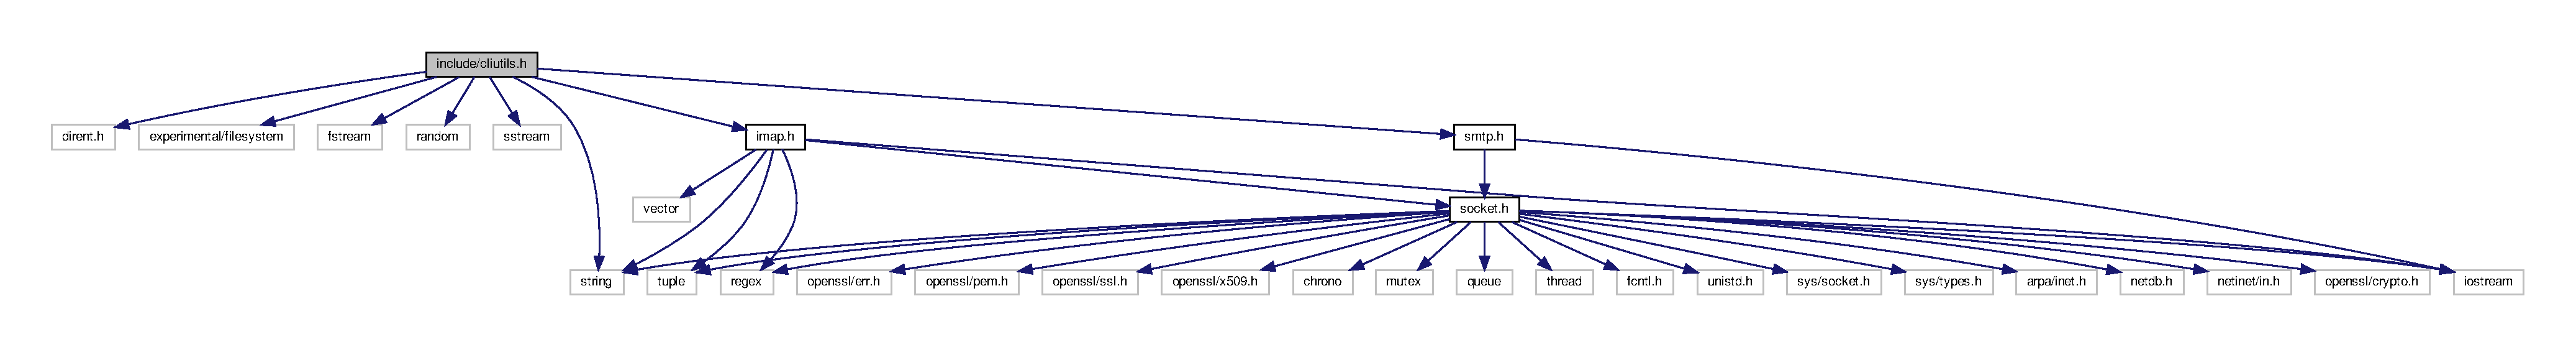
\includegraphics[width=350pt]{cliutils_8h__incl}
\end{center}
\end{figure}
This graph shows which files directly or indirectly include this file\+:
\nopagebreak
\begin{figure}[H]
\begin{center}
\leavevmode
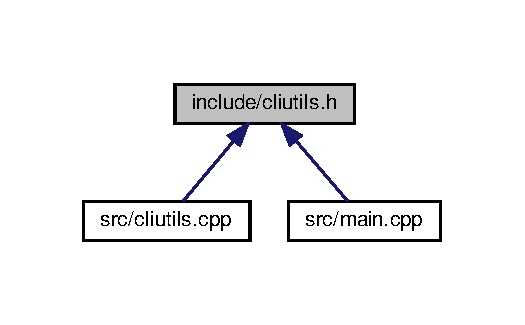
\includegraphics[width=252pt]{cliutils_8h__dep__incl}
\end{center}
\end{figure}
\subsection*{Classes}
\begin{DoxyCompactItemize}
\item 
struct \hyperlink{structconfig}{config}
\begin{DoxyCompactList}\small\item\em Config structure used to store the details of the server and user. \end{DoxyCompactList}\end{DoxyCompactItemize}
\subsection*{Functions}
\begin{DoxyCompactItemize}
\item 
std\+::string \hyperlink{cliutils_8h_a89975953b7d9023cb11eedbd419de5e5}{M\+A\+I\+L\+\_\+\+P\+A\+TH} ()
\begin{DoxyCompactList}\small\item\em M\+A\+I\+L\+\_\+\+P\+A\+TH. \end{DoxyCompactList}\item 
void \hyperlink{cliutils_8h_a972a43991062ce2daf1f0de24fbd6a67}{Get\+Req\+Dirs} (const std\+::string \&path, std\+::vector$<$ std\+::string $>$ \&dirs)
\begin{DoxyCompactList}\small\item\em Get directories. \end{DoxyCompactList}\item 
std\+::string \hyperlink{cliutils_8h_af6f98acaa9bd103b6b455201fd713d34}{tolowercase} (const std\+::string \&s)
\begin{DoxyCompactList}\small\item\em Convert string to lowercase. \end{DoxyCompactList}\item 
bool \hyperlink{cliutils_8h_a0f8558066434c355e9ad6f4bcce90f17}{cliutils\+::sync} (\hyperlink{classIMAPConnection}{I\+M\+A\+P\+Connection} \&imap)
\begin{DoxyCompactList}\small\item\em Syncs the messages from the server. \end{DoxyCompactList}\item 
bool \hyperlink{cliutils_8h_abc7c1b32e5dcb85bbe3fcbabd5f5b969}{cliutils\+::send\+Mail} (\hyperlink{structconfig}{config} \&\hyperlink{structconfig}{config}, const std\+::string \&to, const std\+::string \&subject, const std\+::string \&msg)
\begin{DoxyCompactList}\small\item\em Send a mail using S\+M\+TP. \end{DoxyCompactList}\item 
bool \hyperlink{cliutils_8h_a98b1e24715d5fa5d12bda3f22bf2a621}{cliutils\+::delete\+Mail} (\hyperlink{classIMAPConnection}{I\+M\+A\+P\+Connection} \&imap, const std\+::string \&mailbox, int uid)
\begin{DoxyCompactList}\small\item\em Deletes a mail. \end{DoxyCompactList}\item 
\hyperlink{structMail}{Mail} \hyperlink{cliutils_8h_a660a0a035059deaf25f87d941ba13497}{cliutils\+::read\+Mail} (const std\+::string \&mailbox, int uid)
\begin{DoxyCompactList}\small\item\em Read a mail. \end{DoxyCompactList}\item 
std\+::vector$<$ \hyperlink{structMail}{Mail} $>$ \hyperlink{cliutils_8h_ad2c2a6c179d4848a8b63d563c835417f}{cliutils\+::get\+Mails} (\hyperlink{classIMAPConnection}{I\+M\+A\+P\+Connection} \&imap, const std\+::string \&mailbox, std\+::vector$<$ int $>$ uids)
\begin{DoxyCompactList}\small\item\em Get Mails from the server. \end{DoxyCompactList}\item 
std\+::vector$<$ int $>$ \hyperlink{cliutils_8h_a6c58669367647ec4677d06c2e021b1fc}{cliutils\+::search\+Mails} (\hyperlink{classIMAPConnection}{I\+M\+A\+P\+Connection} \&imap, const std\+::string \&mailbox, const std\+::string \&from, const std\+::string \&to, const std\+::string \&subject, const std\+::string \&text, const std\+::string \&nottext, const std\+::string \&since, const std\+::string \&before)
\begin{DoxyCompactList}\small\item\em Search mails using imap search command. \end{DoxyCompactList}\item 
bool \hyperlink{cliutils_8h_a4d1b5e281c24accf9ff70a4ea7cb32cd}{cliutils\+::create\+Mailbox} (\hyperlink{classIMAPConnection}{I\+M\+A\+P\+Connection} \&imap, const std\+::string \&mailbox)
\begin{DoxyCompactList}\small\item\em Create mailbox. \end{DoxyCompactList}\item 
bool \hyperlink{cliutils_8h_abc861e9fc4c19119f77ec46f8b710f39}{cliutils\+::delete\+Mailbox} (\hyperlink{classIMAPConnection}{I\+M\+A\+P\+Connection} \&imap, const std\+::string \&mailbox)
\begin{DoxyCompactList}\small\item\em Delete mailbox. \end{DoxyCompactList}\item 
bool \hyperlink{cliutils_8h_ac5793a0243f3dacf73137a699a04976c}{cliutils\+::rename\+Mailbox} (\hyperlink{classIMAPConnection}{I\+M\+A\+P\+Connection} \&imap, const std\+::string \&oldmailbox, const std\+::string \&newmailbox)
\begin{DoxyCompactList}\small\item\em Rename mailbox. \end{DoxyCompactList}\item 
bool \hyperlink{cliutils_8h_a9d223cc0393c24be2ba5c5d2cc2880d0}{cliutils\+::move\+Mail} (\hyperlink{classIMAPConnection}{I\+M\+A\+P\+Connection} \&imap, const std\+::string \&oldmailbox, int uid, const std\+::string \&newmailbox)
\begin{DoxyCompactList}\small\item\em Move mail. \end{DoxyCompactList}\item 
std\+::vector$<$ std\+::string $>$ \hyperlink{cliutils_8h_ae49892a449492f76ddb2319534659072}{cliutils\+::get\+Mailboxes} ()
\begin{DoxyCompactList}\small\item\em List mailboxes. \end{DoxyCompactList}\item 
bool \hyperlink{cliutils_8h_aa963e82596d70aacc2a79a1829ee4b8d}{cliutils\+::noop} (\hyperlink{classIMAPConnection}{I\+M\+A\+P\+Connection} \&imap)
\begin{DoxyCompactList}\small\item\em Noop imap. \end{DoxyCompactList}\end{DoxyCompactItemize}


\subsection{Function Documentation}
\mbox{\Hypertarget{cliutils_8h_file_a4d1b5e281c24accf9ff70a4ea7cb32cd}\label{cliutils_8h_file_a4d1b5e281c24accf9ff70a4ea7cb32cd}} 
\index{cliutils.\+h@{cliutils.\+h}!create\+Mailbox@{create\+Mailbox}}
\index{create\+Mailbox@{create\+Mailbox}!cliutils.\+h@{cliutils.\+h}}
\subsubsection{\texorpdfstring{create\+Mailbox()}{createMailbox()}}
{\footnotesize\ttfamily bool cliutils\+::create\+Mailbox (\begin{DoxyParamCaption}\item[{\hyperlink{classIMAPConnection}{I\+M\+A\+P\+Connection} \&}]{imap,  }\item[{const std\+::string \&}]{mailbox }\end{DoxyParamCaption})}



Create mailbox. 

Create a mailbox


\begin{DoxyParams}{Parameters}
{\em imap} & \hyperlink{classIMAPConnection}{I\+M\+A\+P\+Connection} object \\
\hline
{\em mailbox} & The mailbix to be created\\
\hline
\end{DoxyParams}
\begin{DoxyReturn}{Returns}
Status whether mailbox is created 
\end{DoxyReturn}
\mbox{\Hypertarget{cliutils_8h_file_a98b1e24715d5fa5d12bda3f22bf2a621}\label{cliutils_8h_file_a98b1e24715d5fa5d12bda3f22bf2a621}} 
\index{cliutils.\+h@{cliutils.\+h}!delete\+Mail@{delete\+Mail}}
\index{delete\+Mail@{delete\+Mail}!cliutils.\+h@{cliutils.\+h}}
\subsubsection{\texorpdfstring{delete\+Mail()}{deleteMail()}}
{\footnotesize\ttfamily bool cliutils\+::delete\+Mail (\begin{DoxyParamCaption}\item[{\hyperlink{classIMAPConnection}{I\+M\+A\+P\+Connection} \&}]{imap,  }\item[{const std\+::string \&}]{mailbox,  }\item[{int}]{uid }\end{DoxyParamCaption})}



Deletes a mail. 

Deletes the mail with given uid from given mailbox


\begin{DoxyParams}{Parameters}
{\em imap} & \hyperlink{classIMAPConnection}{I\+M\+A\+P\+Connection} to send the delete command \\
\hline
{\em mailbox} & The mailbox from which the mail is to be deleted \\
\hline
{\em uid} & The uid of the mail to be deleted \\
\hline
\end{DoxyParams}
\begin{DoxyReturn}{Returns}
Whether the mail was sucessfully deleted or not 
\end{DoxyReturn}
\mbox{\Hypertarget{cliutils_8h_file_abc861e9fc4c19119f77ec46f8b710f39}\label{cliutils_8h_file_abc861e9fc4c19119f77ec46f8b710f39}} 
\index{cliutils.\+h@{cliutils.\+h}!delete\+Mailbox@{delete\+Mailbox}}
\index{delete\+Mailbox@{delete\+Mailbox}!cliutils.\+h@{cliutils.\+h}}
\subsubsection{\texorpdfstring{delete\+Mailbox()}{deleteMailbox()}}
{\footnotesize\ttfamily bool cliutils\+::delete\+Mailbox (\begin{DoxyParamCaption}\item[{\hyperlink{classIMAPConnection}{I\+M\+A\+P\+Connection} \&}]{imap,  }\item[{const std\+::string \&}]{mailbox }\end{DoxyParamCaption})}



Delete mailbox. 

Delete a mailbox


\begin{DoxyParams}{Parameters}
{\em imap} & \hyperlink{classIMAPConnection}{I\+M\+A\+P\+Connection} object \\
\hline
{\em mailbox} & The mailbox to be deleted\\
\hline
\end{DoxyParams}
\begin{DoxyReturn}{Returns}
Status whether mailbox is deleted 
\end{DoxyReturn}
\mbox{\Hypertarget{cliutils_8h_file_ae49892a449492f76ddb2319534659072}\label{cliutils_8h_file_ae49892a449492f76ddb2319534659072}} 
\index{cliutils.\+h@{cliutils.\+h}!get\+Mailboxes@{get\+Mailboxes}}
\index{get\+Mailboxes@{get\+Mailboxes}!cliutils.\+h@{cliutils.\+h}}
\subsubsection{\texorpdfstring{get\+Mailboxes()}{getMailboxes()}}
{\footnotesize\ttfamily std\+::vector$<$ std\+::string $>$ cliutils\+::get\+Mailboxes (\begin{DoxyParamCaption}{ }\end{DoxyParamCaption})}



List mailboxes. 

List all the mailboxes available offline \begin{DoxyReturn}{Returns}
List of mailboxed 
\end{DoxyReturn}
\mbox{\Hypertarget{cliutils_8h_file_ad2c2a6c179d4848a8b63d563c835417f}\label{cliutils_8h_file_ad2c2a6c179d4848a8b63d563c835417f}} 
\index{cliutils.\+h@{cliutils.\+h}!get\+Mails@{get\+Mails}}
\index{get\+Mails@{get\+Mails}!cliutils.\+h@{cliutils.\+h}}
\subsubsection{\texorpdfstring{get\+Mails()}{getMails()}}
{\footnotesize\ttfamily std\+::vector$<$ \hyperlink{structMail}{Mail} $>$ cliutils\+::get\+Mails (\begin{DoxyParamCaption}\item[{\hyperlink{classIMAPConnection}{I\+M\+A\+P\+Connection} \&}]{imap,  }\item[{const std\+::string \&}]{mailbox,  }\item[{std\+::vector$<$ int $>$}]{uids }\end{DoxyParamCaption})}



Get Mails from the server. 

Fetches mails from imap server in a given mailbox


\begin{DoxyParams}{Parameters}
{\em imap} & \hyperlink{classIMAPConnection}{I\+M\+A\+P\+Connection} object \\
\hline
{\em mailbox} & Mailbox from which mails are to be fetched \\
\hline
{\em uids} & The uids of the mails which are to be fetched \\
\hline
\end{DoxyParams}
\begin{DoxyReturn}{Returns}
Vector of \hyperlink{structMail}{Mail} objects. 
\end{DoxyReturn}
\mbox{\Hypertarget{cliutils_8h_a972a43991062ce2daf1f0de24fbd6a67}\label{cliutils_8h_a972a43991062ce2daf1f0de24fbd6a67}} 
\index{cliutils.\+h@{cliutils.\+h}!Get\+Req\+Dirs@{Get\+Req\+Dirs}}
\index{Get\+Req\+Dirs@{Get\+Req\+Dirs}!cliutils.\+h@{cliutils.\+h}}
\subsubsection{\texorpdfstring{Get\+Req\+Dirs()}{GetReqDirs()}}
{\footnotesize\ttfamily void Get\+Req\+Dirs (\begin{DoxyParamCaption}\item[{const std\+::string \&}]{path,  }\item[{std\+::vector$<$ std\+::string $>$ \&}]{dirs }\end{DoxyParamCaption})}



Get directories. 

List all directories stored in path


\begin{DoxyParams}{Parameters}
{\em path} & Path to search directories for \\
\hline
{\em dirs} & Appends directories to this vector \\
\hline
\end{DoxyParams}
\mbox{\Hypertarget{cliutils_8h_a89975953b7d9023cb11eedbd419de5e5}\label{cliutils_8h_a89975953b7d9023cb11eedbd419de5e5}} 
\index{cliutils.\+h@{cliutils.\+h}!M\+A\+I\+L\+\_\+\+P\+A\+TH@{M\+A\+I\+L\+\_\+\+P\+A\+TH}}
\index{M\+A\+I\+L\+\_\+\+P\+A\+TH@{M\+A\+I\+L\+\_\+\+P\+A\+TH}!cliutils.\+h@{cliutils.\+h}}
\subsubsection{\texorpdfstring{M\+A\+I\+L\+\_\+\+P\+A\+T\+H()}{MAIL\_PATH()}}
{\footnotesize\ttfamily std\+::string M\+A\+I\+L\+\_\+\+P\+A\+TH (\begin{DoxyParamCaption}{ }\end{DoxyParamCaption})}



M\+A\+I\+L\+\_\+\+P\+A\+TH. 

Offline mail path i.\+e. {\ttfamily \$\+H\+O\+ME/.mailc} \begin{DoxyReturn}{Returns}
Returns the offline mail path 
\end{DoxyReturn}
\mbox{\Hypertarget{cliutils_8h_file_a9d223cc0393c24be2ba5c5d2cc2880d0}\label{cliutils_8h_file_a9d223cc0393c24be2ba5c5d2cc2880d0}} 
\index{cliutils.\+h@{cliutils.\+h}!move\+Mail@{move\+Mail}}
\index{move\+Mail@{move\+Mail}!cliutils.\+h@{cliutils.\+h}}
\subsubsection{\texorpdfstring{move\+Mail()}{moveMail()}}
{\footnotesize\ttfamily bool cliutils\+::move\+Mail (\begin{DoxyParamCaption}\item[{\hyperlink{classIMAPConnection}{I\+M\+A\+P\+Connection} \&}]{imap,  }\item[{const std\+::string \&}]{oldmailbox,  }\item[{int}]{uid,  }\item[{const std\+::string \&}]{newmailbox }\end{DoxyParamCaption})}



Move mail. 

Move a mail from one mailbox to another


\begin{DoxyParams}{Parameters}
{\em imap} & \hyperlink{classIMAPConnection}{I\+M\+A\+P\+Connection} object \\
\hline
{\em oldmailbox} & Current mailbox of the mail \\
\hline
{\em uid} & The uid of the mail \\
\hline
{\em newmailbox} & Mailbox to move the mail into \\
\hline
\end{DoxyParams}
\begin{DoxyReturn}{Returns}
Status whether the mail was moved or not 
\end{DoxyReturn}
\mbox{\Hypertarget{cliutils_8h_file_aa963e82596d70aacc2a79a1829ee4b8d}\label{cliutils_8h_file_aa963e82596d70aacc2a79a1829ee4b8d}} 
\index{cliutils.\+h@{cliutils.\+h}!noop@{noop}}
\index{noop@{noop}!cliutils.\+h@{cliutils.\+h}}
\subsubsection{\texorpdfstring{noop()}{noop()}}
{\footnotesize\ttfamily bool cliutils\+::noop (\begin{DoxyParamCaption}\item[{\hyperlink{classIMAPConnection}{I\+M\+A\+P\+Connection} \&}]{imap }\end{DoxyParamCaption})}



Noop imap. 

Continue connection with imap server \begin{DoxyReturn}{Returns}
Status whether noop was successful 
\end{DoxyReturn}
\mbox{\Hypertarget{cliutils_8h_file_a660a0a035059deaf25f87d941ba13497}\label{cliutils_8h_file_a660a0a035059deaf25f87d941ba13497}} 
\index{cliutils.\+h@{cliutils.\+h}!read\+Mail@{read\+Mail}}
\index{read\+Mail@{read\+Mail}!cliutils.\+h@{cliutils.\+h}}
\subsubsection{\texorpdfstring{read\+Mail()}{readMail()}}
{\footnotesize\ttfamily \hyperlink{structMail}{Mail} cliutils\+::read\+Mail (\begin{DoxyParamCaption}\item[{const std\+::string \&}]{mailbox,  }\item[{int}]{uid }\end{DoxyParamCaption})}



Read a mail. 

Read an email stored offline


\begin{DoxyParams}{Parameters}
{\em mailbox} & The mailbox from which the mail is to be read \\
\hline
{\em uid} & The uid of the mail\\
\hline
\end{DoxyParams}
\begin{DoxyReturn}{Returns}
The \hyperlink{structMail}{Mail} object containg the mail details 
\end{DoxyReturn}
\mbox{\Hypertarget{cliutils_8h_file_ac5793a0243f3dacf73137a699a04976c}\label{cliutils_8h_file_ac5793a0243f3dacf73137a699a04976c}} 
\index{cliutils.\+h@{cliutils.\+h}!rename\+Mailbox@{rename\+Mailbox}}
\index{rename\+Mailbox@{rename\+Mailbox}!cliutils.\+h@{cliutils.\+h}}
\subsubsection{\texorpdfstring{rename\+Mailbox()}{renameMailbox()}}
{\footnotesize\ttfamily bool cliutils\+::rename\+Mailbox (\begin{DoxyParamCaption}\item[{\hyperlink{classIMAPConnection}{I\+M\+A\+P\+Connection} \&}]{imap,  }\item[{const std\+::string \&}]{oldmailbox,  }\item[{const std\+::string \&}]{newmailbox }\end{DoxyParamCaption})}



Rename mailbox. 

Rename a mailbox


\begin{DoxyParams}{Parameters}
{\em imap} & \hyperlink{classIMAPConnection}{I\+M\+A\+P\+Connection} object \\
\hline
{\em oldmailbox} & Old name of the mailbox \\
\hline
{\em newmailbox} & New name of the mailbox \\
\hline
\end{DoxyParams}
\begin{DoxyReturn}{Returns}
Status whether the mailbox was renamed 
\end{DoxyReturn}
\mbox{\Hypertarget{cliutils_8h_file_a6c58669367647ec4677d06c2e021b1fc}\label{cliutils_8h_file_a6c58669367647ec4677d06c2e021b1fc}} 
\index{cliutils.\+h@{cliutils.\+h}!search\+Mails@{search\+Mails}}
\index{search\+Mails@{search\+Mails}!cliutils.\+h@{cliutils.\+h}}
\subsubsection{\texorpdfstring{search\+Mails()}{searchMails()}}
{\footnotesize\ttfamily std\+::vector$<$ int $>$ cliutils\+::search\+Mails (\begin{DoxyParamCaption}\item[{\hyperlink{classIMAPConnection}{I\+M\+A\+P\+Connection} \&}]{imap,  }\item[{const std\+::string \&}]{mailbox,  }\item[{const std\+::string \&}]{from,  }\item[{const std\+::string \&}]{to,  }\item[{const std\+::string \&}]{subject,  }\item[{const std\+::string \&}]{text,  }\item[{const std\+::string \&}]{nottext,  }\item[{const std\+::string \&}]{since,  }\item[{const std\+::string \&}]{before }\end{DoxyParamCaption})}



Search mails using imap search command. 

Search mails based on various search filters


\begin{DoxyParams}{Parameters}
{\em imap} & I\+M\+A\+P\+Connectio object \\
\hline
{\em mailbox} & Mailbox to search mails from \\
\hline
{\em from} & Search mails received from \\
\hline
{\em to} & Search mails sent to \\
\hline
{\em subject} & Search mails containg a text in subject \\
\hline
{\em text} & Search the mails containing a text in body \\
\hline
{\em nottext} & Search the mails not containing a text \\
\hline
{\em since} & Search the mails since a date \\
\hline
{\em before} & Search the mails before a date \\
\hline
\end{DoxyParams}
\begin{DoxyReturn}{Returns}
All the uids of the mail matching the search filters 
\end{DoxyReturn}
\mbox{\Hypertarget{cliutils_8h_file_abc7c1b32e5dcb85bbe3fcbabd5f5b969}\label{cliutils_8h_file_abc7c1b32e5dcb85bbe3fcbabd5f5b969}} 
\index{cliutils.\+h@{cliutils.\+h}!send\+Mail@{send\+Mail}}
\index{send\+Mail@{send\+Mail}!cliutils.\+h@{cliutils.\+h}}
\subsubsection{\texorpdfstring{send\+Mail()}{sendMail()}}
{\footnotesize\ttfamily bool cliutils\+::send\+Mail (\begin{DoxyParamCaption}\item[{\hyperlink{structconfig}{config} \&}]{config,  }\item[{const std\+::string \&}]{to,  }\item[{const std\+::string \&}]{subject,  }\item[{const std\+::string \&}]{msg }\end{DoxyParamCaption})}



Send a mail using S\+M\+TP. 

This function creates an S\+M\+TP Connection and send the mail to using S\+M\+TP protocol.


\begin{DoxyParams}{Parameters}
{\em config} & Details about server and user. \\
\hline
{\em to} & To mail address \\
\hline
{\em subject} & Subject of the mail \\
\hline
{\em msg} & The body of the mail \\
\hline
\end{DoxyParams}
\begin{DoxyReturn}{Returns}
Whether the mail was sent successfully or not. 
\end{DoxyReturn}
\mbox{\Hypertarget{cliutils_8h_file_a0f8558066434c355e9ad6f4bcce90f17}\label{cliutils_8h_file_a0f8558066434c355e9ad6f4bcce90f17}} 
\index{cliutils.\+h@{cliutils.\+h}!sync@{sync}}
\index{sync@{sync}!cliutils.\+h@{cliutils.\+h}}
\subsubsection{\texorpdfstring{sync()}{sync()}}
{\footnotesize\ttfamily bool cliutils\+::sync (\begin{DoxyParamCaption}\item[{\hyperlink{classIMAPConnection}{I\+M\+A\+P\+Connection} \&}]{imap }\end{DoxyParamCaption})}



Syncs the messages from the server. 

This function syncs the messages from the server and are stored \$\+H\+O\+ME/.mailc directory


\begin{DoxyParams}{Parameters}
{\em imap} & \hyperlink{classIMAPConnection}{I\+M\+A\+P\+Connection} object to sync messages from \\
\hline
\end{DoxyParams}
\begin{DoxyReturn}{Returns}
Whether the sync was successful or not. 
\end{DoxyReturn}
\mbox{\Hypertarget{cliutils_8h_af6f98acaa9bd103b6b455201fd713d34}\label{cliutils_8h_af6f98acaa9bd103b6b455201fd713d34}} 
\index{cliutils.\+h@{cliutils.\+h}!tolowercase@{tolowercase}}
\index{tolowercase@{tolowercase}!cliutils.\+h@{cliutils.\+h}}
\subsubsection{\texorpdfstring{tolowercase()}{tolowercase()}}
{\footnotesize\ttfamily std\+::string tolowercase (\begin{DoxyParamCaption}\item[{const std\+::string \&}]{s }\end{DoxyParamCaption})}



Convert string to lowercase. 


\begin{DoxyParams}{Parameters}
{\em s} & String object \\
\hline
\end{DoxyParams}
\begin{DoxyReturn}{Returns}
Lowercase of the input string 
\end{DoxyReturn}

\hypertarget{imap_8h}{}\section{include/imap.h File Reference}
\label{imap_8h}\index{include/imap.\+h@{include/imap.\+h}}
{\ttfamily \#include $<$iostream$>$}\newline
{\ttfamily \#include $<$regex$>$}\newline
{\ttfamily \#include $<$string$>$}\newline
{\ttfamily \#include $<$tuple$>$}\newline
{\ttfamily \#include $<$vector$>$}\newline
{\ttfamily \#include \char`\"{}socket.\+h\char`\"{}}\newline
Include dependency graph for imap.\+h\+:
\nopagebreak
\begin{figure}[H]
\begin{center}
\leavevmode
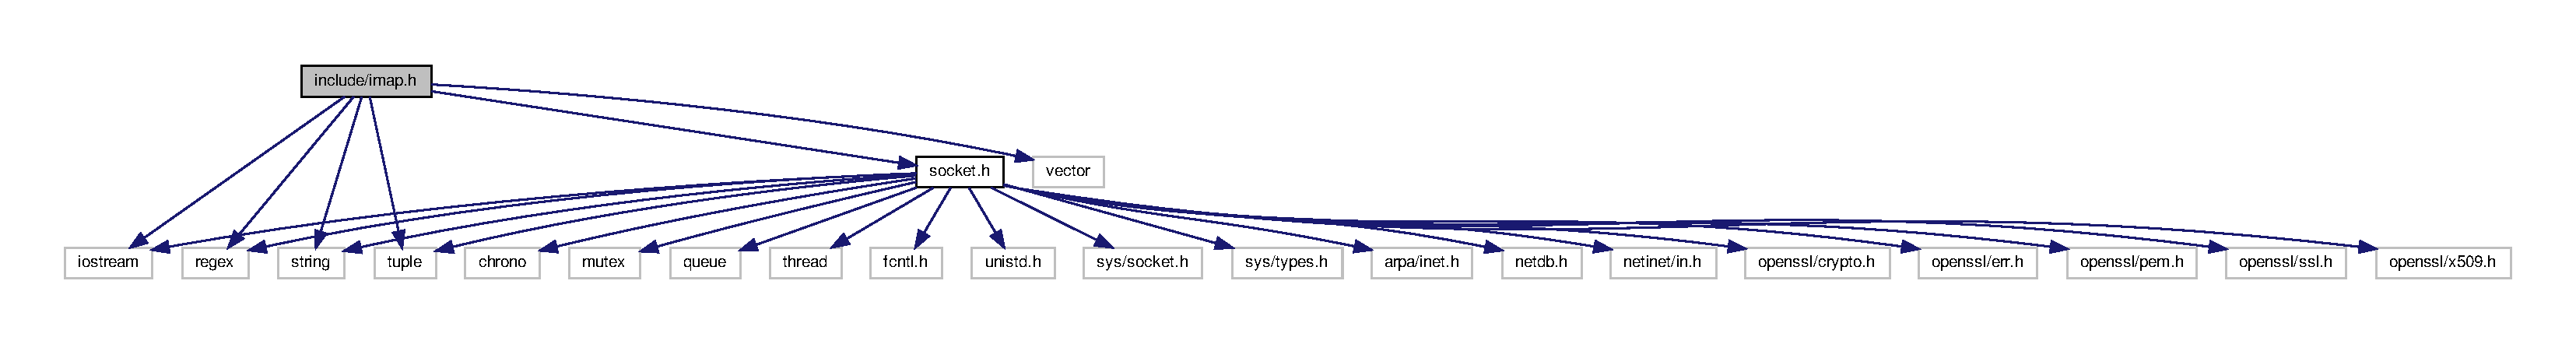
\includegraphics[width=350pt]{imap_8h__incl}
\end{center}
\end{figure}
This graph shows which files directly or indirectly include this file\+:
\nopagebreak
\begin{figure}[H]
\begin{center}
\leavevmode
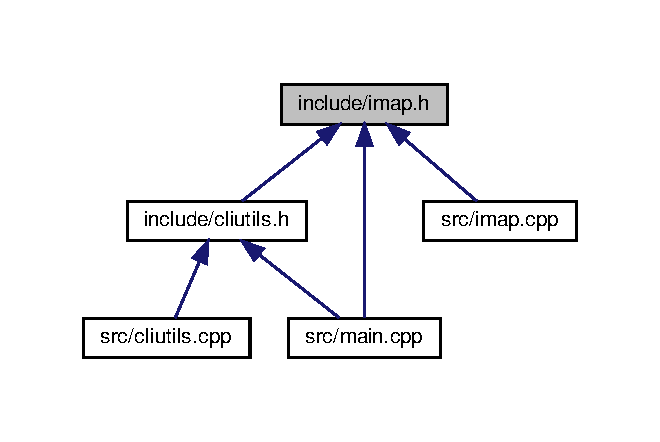
\includegraphics[width=317pt]{imap_8h__dep__incl}
\end{center}
\end{figure}
\subsection*{Classes}
\begin{DoxyCompactItemize}
\item 
struct \hyperlink{structMail}{Mail}
\begin{DoxyCompactList}\small\item\em \hyperlink{structMail}{Mail} structure. \end{DoxyCompactList}\item 
class \hyperlink{classIMAPConnection}{I\+M\+A\+P\+Connection}
\begin{DoxyCompactList}\small\item\em \hyperlink{classIMAPConnection}{I\+M\+A\+P\+Connection} class. \end{DoxyCompactList}\end{DoxyCompactItemize}

\hypertarget{smtp_8h}{}\section{include/smtp.h File Reference}
\label{smtp_8h}\index{include/smtp.\+h@{include/smtp.\+h}}
{\ttfamily \#include $<$iostream$>$}\newline
{\ttfamily \#include \char`\"{}socket.\+h\char`\"{}}\newline
Include dependency graph for smtp.\+h\+:\nopagebreak
\begin{figure}[H]
\begin{center}
\leavevmode
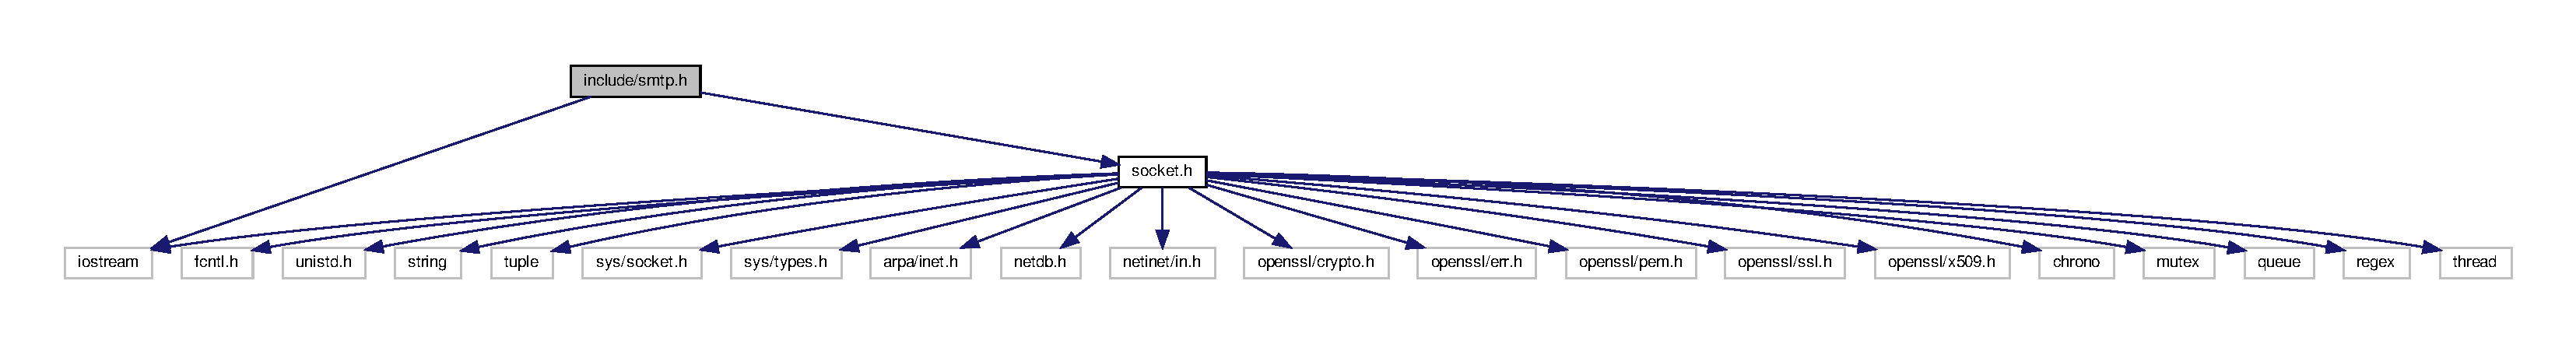
\includegraphics[width=350pt]{smtp_8h__incl}
\end{center}
\end{figure}
This graph shows which files directly or indirectly include this file\+:\nopagebreak
\begin{figure}[H]
\begin{center}
\leavevmode
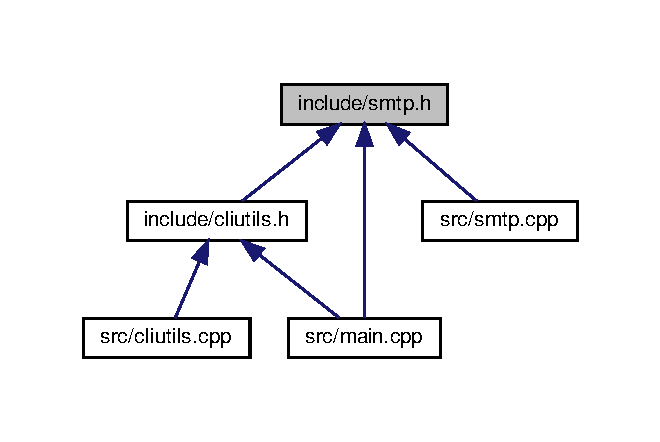
\includegraphics[width=317pt]{smtp_8h__dep__incl}
\end{center}
\end{figure}
\subsection*{Classes}
\begin{DoxyCompactItemize}
\item 
class \hyperlink{classSMTPConnection}{S\+M\+T\+P\+Connection}
\begin{DoxyCompactList}\small\item\em \hyperlink{classSMTPConnection}{S\+M\+T\+P\+Connection} class. \end{DoxyCompactList}\end{DoxyCompactItemize}

\hypertarget{socket_8h}{}\section{include/socket.h File Reference}
\label{socket_8h}\index{include/socket.\+h@{include/socket.\+h}}
{\ttfamily \#include $<$fcntl.\+h$>$}\newline
{\ttfamily \#include $<$unistd.\+h$>$}\newline
{\ttfamily \#include $<$string$>$}\newline
{\ttfamily \#include $<$tuple$>$}\newline
{\ttfamily \#include $<$sys/socket.\+h$>$}\newline
{\ttfamily \#include $<$sys/types.\+h$>$}\newline
{\ttfamily \#include $<$arpa/inet.\+h$>$}\newline
{\ttfamily \#include $<$netdb.\+h$>$}\newline
{\ttfamily \#include $<$netinet/in.\+h$>$}\newline
{\ttfamily \#include $<$openssl/crypto.\+h$>$}\newline
{\ttfamily \#include $<$openssl/err.\+h$>$}\newline
{\ttfamily \#include $<$openssl/pem.\+h$>$}\newline
{\ttfamily \#include $<$openssl/ssl.\+h$>$}\newline
{\ttfamily \#include $<$openssl/x509.\+h$>$}\newline
{\ttfamily \#include $<$chrono$>$}\newline
{\ttfamily \#include $<$iostream$>$}\newline
{\ttfamily \#include $<$mutex$>$}\newline
{\ttfamily \#include $<$queue$>$}\newline
{\ttfamily \#include $<$regex$>$}\newline
{\ttfamily \#include $<$thread$>$}\newline
Include dependency graph for socket.\+h\+:\nopagebreak
\begin{figure}[H]
\begin{center}
\leavevmode
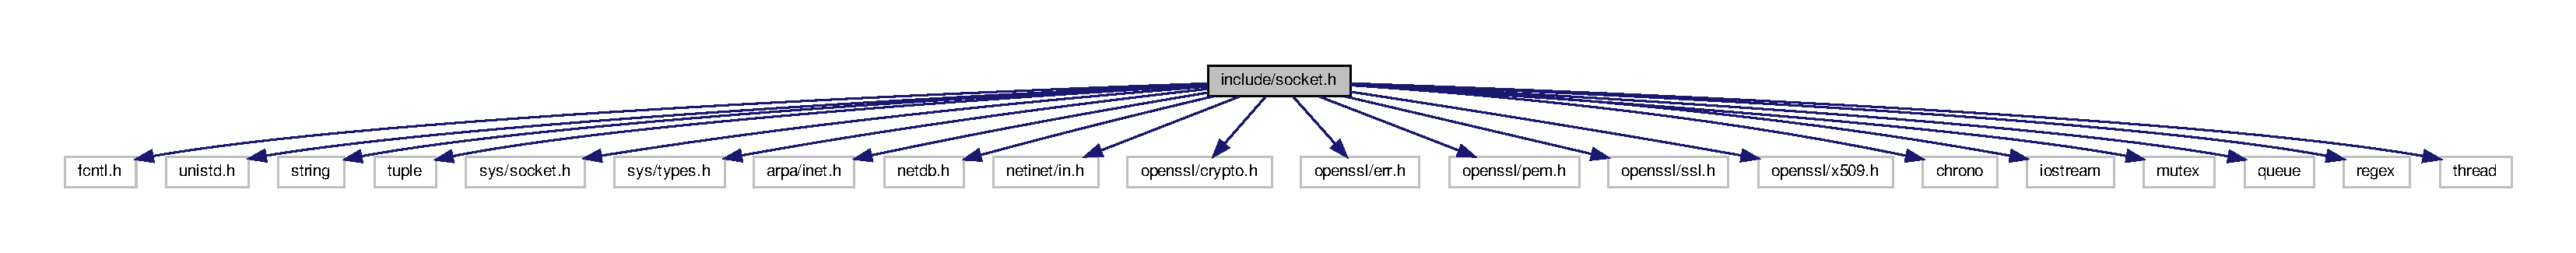
\includegraphics[width=350pt]{socket_8h__incl}
\end{center}
\end{figure}
This graph shows which files directly or indirectly include this file\+:\nopagebreak
\begin{figure}[H]
\begin{center}
\leavevmode
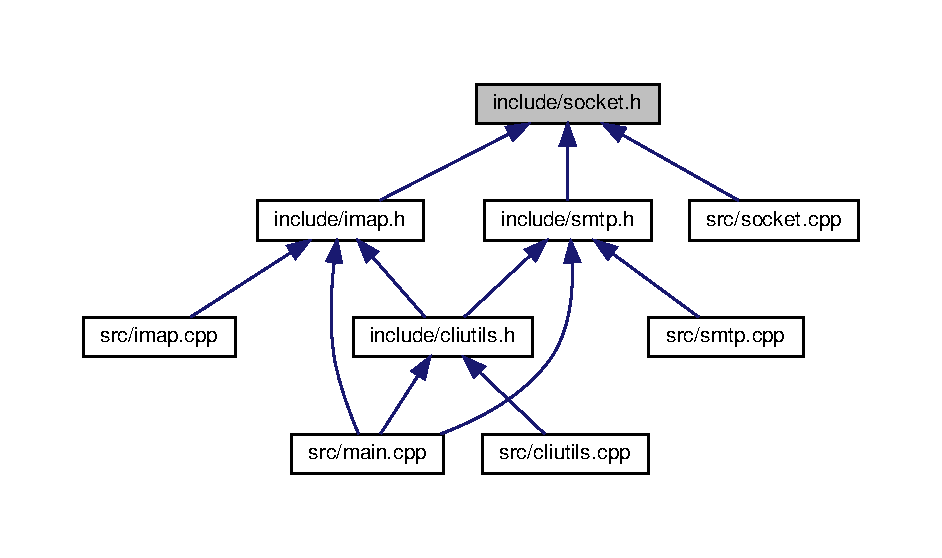
\includegraphics[width=350pt]{socket_8h__dep__incl}
\end{center}
\end{figure}
\subsection*{Classes}
\begin{DoxyCompactItemize}
\item 
class \hyperlink{classSocket}{Socket}
\begin{DoxyCompactList}\small\item\em \hyperlink{classSocket}{Socket} class. \end{DoxyCompactList}\end{DoxyCompactItemize}

\hypertarget{utils_8h}{}\section{include/utils.h File Reference}
\label{utils_8h}\index{include/utils.\+h@{include/utils.\+h}}
{\ttfamily \#include $<$string$>$}\newline
Include dependency graph for utils.\+h\+:
\nopagebreak
\begin{figure}[H]
\begin{center}
\leavevmode
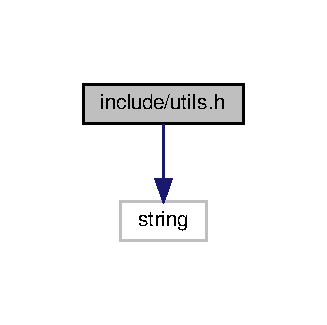
\includegraphics[width=157pt]{utils_8h__incl}
\end{center}
\end{figure}
This graph shows which files directly or indirectly include this file\+:
\nopagebreak
\begin{figure}[H]
\begin{center}
\leavevmode
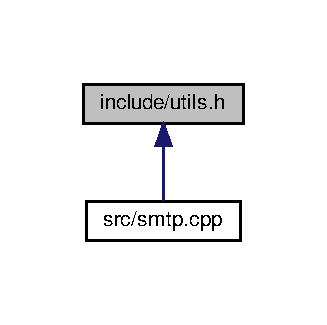
\includegraphics[width=157pt]{utils_8h__dep__incl}
\end{center}
\end{figure}

\hypertarget{cliutils_8cpp}{}\section{src/cliutils.cpp File Reference}
\label{cliutils_8cpp}\index{src/cliutils.\+cpp@{src/cliutils.\+cpp}}
{\ttfamily \#include \char`\"{}cliutils.\+h\char`\"{}}\newline
{\ttfamily \#include $<$algorithm$>$}\newline
{\ttfamily \#include $<$cstdlib$>$}\newline
Include dependency graph for cliutils.\+cpp\+:\nopagebreak
\begin{figure}[H]
\begin{center}
\leavevmode
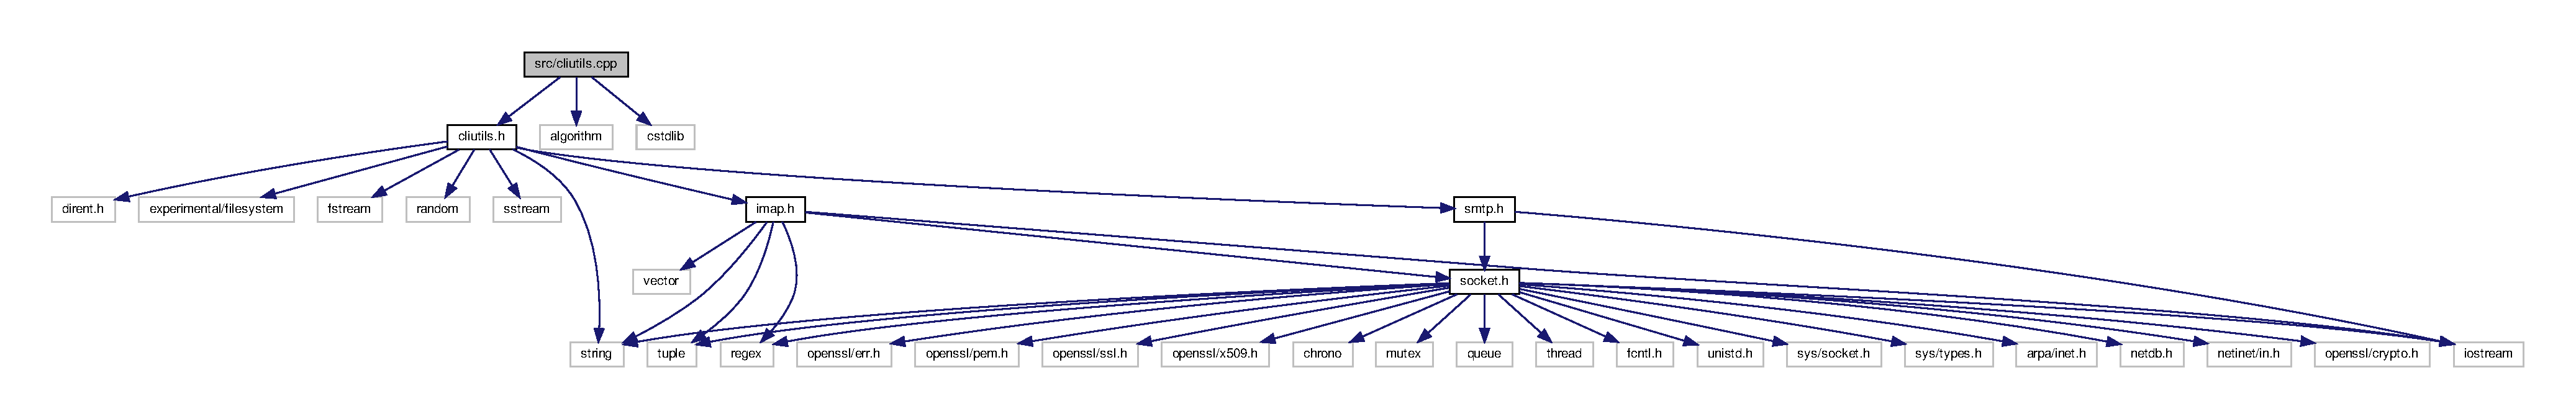
\includegraphics[width=350pt]{cliutils_8cpp__incl}
\end{center}
\end{figure}
\subsection*{Functions}
\begin{DoxyCompactItemize}
\item 
std\+::string \hyperlink{cliutils_8cpp_a89975953b7d9023cb11eedbd419de5e5}{M\+A\+I\+L\+\_\+\+P\+A\+TH} ()
\begin{DoxyCompactList}\small\item\em M\+A\+I\+L\+\_\+\+P\+A\+TH. \end{DoxyCompactList}\item 
void \hyperlink{cliutils_8cpp_a972a43991062ce2daf1f0de24fbd6a67}{Get\+Req\+Dirs} (const std\+::string \&path, std\+::vector$<$ std\+::string $>$ \&dirs)
\begin{DoxyCompactList}\small\item\em Get directories. \end{DoxyCompactList}\item 
std\+::string \hyperlink{cliutils_8cpp_af6f98acaa9bd103b6b455201fd713d34}{tolowercase} (const std\+::string \&s)
\begin{DoxyCompactList}\small\item\em Convert string to lowercase. \end{DoxyCompactList}\item 
\mbox{\Hypertarget{cliutils_8cpp_adf7de668fd10266afe331f579a8178ee}\label{cliutils_8cpp_adf7de668fd10266afe331f579a8178ee}} 
std\+::mt19937 \hyperlink{cliutils_8cpp_adf7de668fd10266afe331f579a8178ee}{rng} (\hyperlink{cliutils_8cpp_a7071b0092ad8c5b57d6cc40c5f803df5}{rd}())
\begin{DoxyCompactList}\small\item\em Random generator object. \end{DoxyCompactList}\end{DoxyCompactItemize}
\subsection*{Variables}
\begin{DoxyCompactItemize}
\item 
\mbox{\Hypertarget{cliutils_8cpp_a7071b0092ad8c5b57d6cc40c5f803df5}\label{cliutils_8cpp_a7071b0092ad8c5b57d6cc40c5f803df5}} 
std\+::random\+\_\+device \hyperlink{cliutils_8cpp_a7071b0092ad8c5b57d6cc40c5f803df5}{rd}
\begin{DoxyCompactList}\small\item\em Random device. \end{DoxyCompactList}\end{DoxyCompactItemize}


\subsection{Function Documentation}
\mbox{\Hypertarget{cliutils_8cpp_a972a43991062ce2daf1f0de24fbd6a67}\label{cliutils_8cpp_a972a43991062ce2daf1f0de24fbd6a67}} 
\index{cliutils.\+cpp@{cliutils.\+cpp}!Get\+Req\+Dirs@{Get\+Req\+Dirs}}
\index{Get\+Req\+Dirs@{Get\+Req\+Dirs}!cliutils.\+cpp@{cliutils.\+cpp}}
\subsubsection{\texorpdfstring{Get\+Req\+Dirs()}{GetReqDirs()}}
{\footnotesize\ttfamily void Get\+Req\+Dirs (\begin{DoxyParamCaption}\item[{const std\+::string \&}]{path,  }\item[{std\+::vector$<$ std\+::string $>$ \&}]{dirs }\end{DoxyParamCaption})}



Get directories. 

List all directories stored in path


\begin{DoxyParams}{Parameters}
{\em path} & Path to search directories for \\
\hline
{\em dirs} & Appends directories to this vector \\
\hline
\end{DoxyParams}
\mbox{\Hypertarget{cliutils_8cpp_a89975953b7d9023cb11eedbd419de5e5}\label{cliutils_8cpp_a89975953b7d9023cb11eedbd419de5e5}} 
\index{cliutils.\+cpp@{cliutils.\+cpp}!M\+A\+I\+L\+\_\+\+P\+A\+TH@{M\+A\+I\+L\+\_\+\+P\+A\+TH}}
\index{M\+A\+I\+L\+\_\+\+P\+A\+TH@{M\+A\+I\+L\+\_\+\+P\+A\+TH}!cliutils.\+cpp@{cliutils.\+cpp}}
\subsubsection{\texorpdfstring{M\+A\+I\+L\+\_\+\+P\+A\+T\+H()}{MAIL\_PATH()}}
{\footnotesize\ttfamily std\+::string M\+A\+I\+L\+\_\+\+P\+A\+TH (\begin{DoxyParamCaption}{ }\end{DoxyParamCaption})}



M\+A\+I\+L\+\_\+\+P\+A\+TH. 

Offline mail path i.\+e. {\ttfamily \$\+H\+O\+ME/.mailc} \begin{DoxyReturn}{Returns}
Returns the offline mail path 
\end{DoxyReturn}
\mbox{\Hypertarget{cliutils_8cpp_af6f98acaa9bd103b6b455201fd713d34}\label{cliutils_8cpp_af6f98acaa9bd103b6b455201fd713d34}} 
\index{cliutils.\+cpp@{cliutils.\+cpp}!tolowercase@{tolowercase}}
\index{tolowercase@{tolowercase}!cliutils.\+cpp@{cliutils.\+cpp}}
\subsubsection{\texorpdfstring{tolowercase()}{tolowercase()}}
{\footnotesize\ttfamily std\+::string tolowercase (\begin{DoxyParamCaption}\item[{const std\+::string \&}]{s }\end{DoxyParamCaption})}



Convert string to lowercase. 


\begin{DoxyParams}{Parameters}
{\em s} & String object \\
\hline
\end{DoxyParams}
\begin{DoxyReturn}{Returns}
Lowercase of the input string 
\end{DoxyReturn}

\hypertarget{imap_8cpp}{}\section{src/imap.cpp File Reference}
\label{imap_8cpp}\index{src/imap.\+cpp@{src/imap.\+cpp}}
{\ttfamily \#include \char`\"{}imap.\+h\char`\"{}}\newline
Include dependency graph for imap.\+cpp\+:
\nopagebreak
\begin{figure}[H]
\begin{center}
\leavevmode
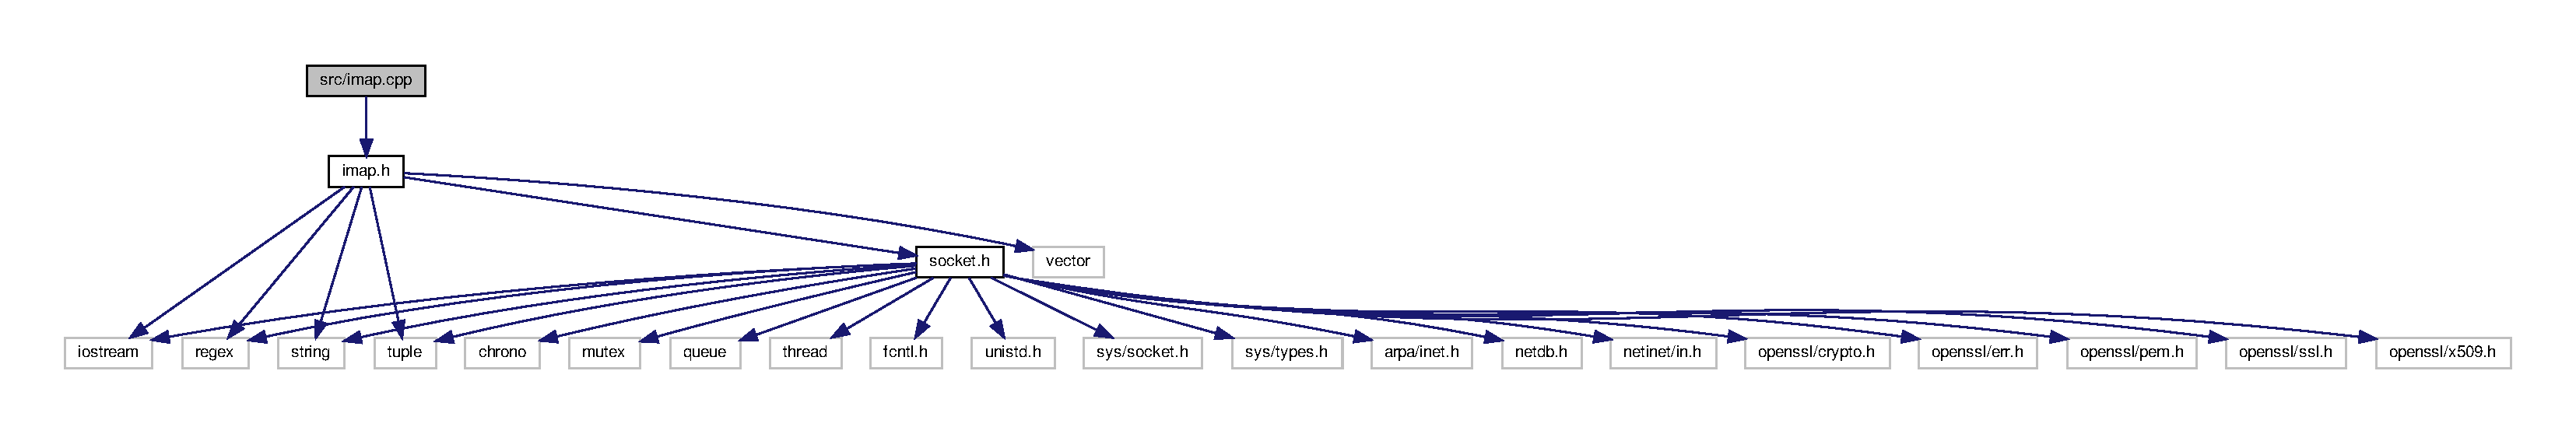
\includegraphics[width=350pt]{imap_8cpp__incl}
\end{center}
\end{figure}

\hypertarget{main_8cpp}{}\section{src/main.cpp File Reference}
\label{main_8cpp}\index{src/main.\+cpp@{src/main.\+cpp}}
{\ttfamily \#include \char`\"{}cliutils.\+h\char`\"{}}\newline
{\ttfamily \#include \char`\"{}imap.\+h\char`\"{}}\newline
{\ttfamily \#include \char`\"{}smtp.\+h\char`\"{}}\newline
{\ttfamily \#include $<$readline/history.\+h$>$}\newline
{\ttfamily \#include $<$readline/readline.\+h$>$}\newline
Include dependency graph for main.\+cpp\+:
\nopagebreak
\begin{figure}[H]
\begin{center}
\leavevmode
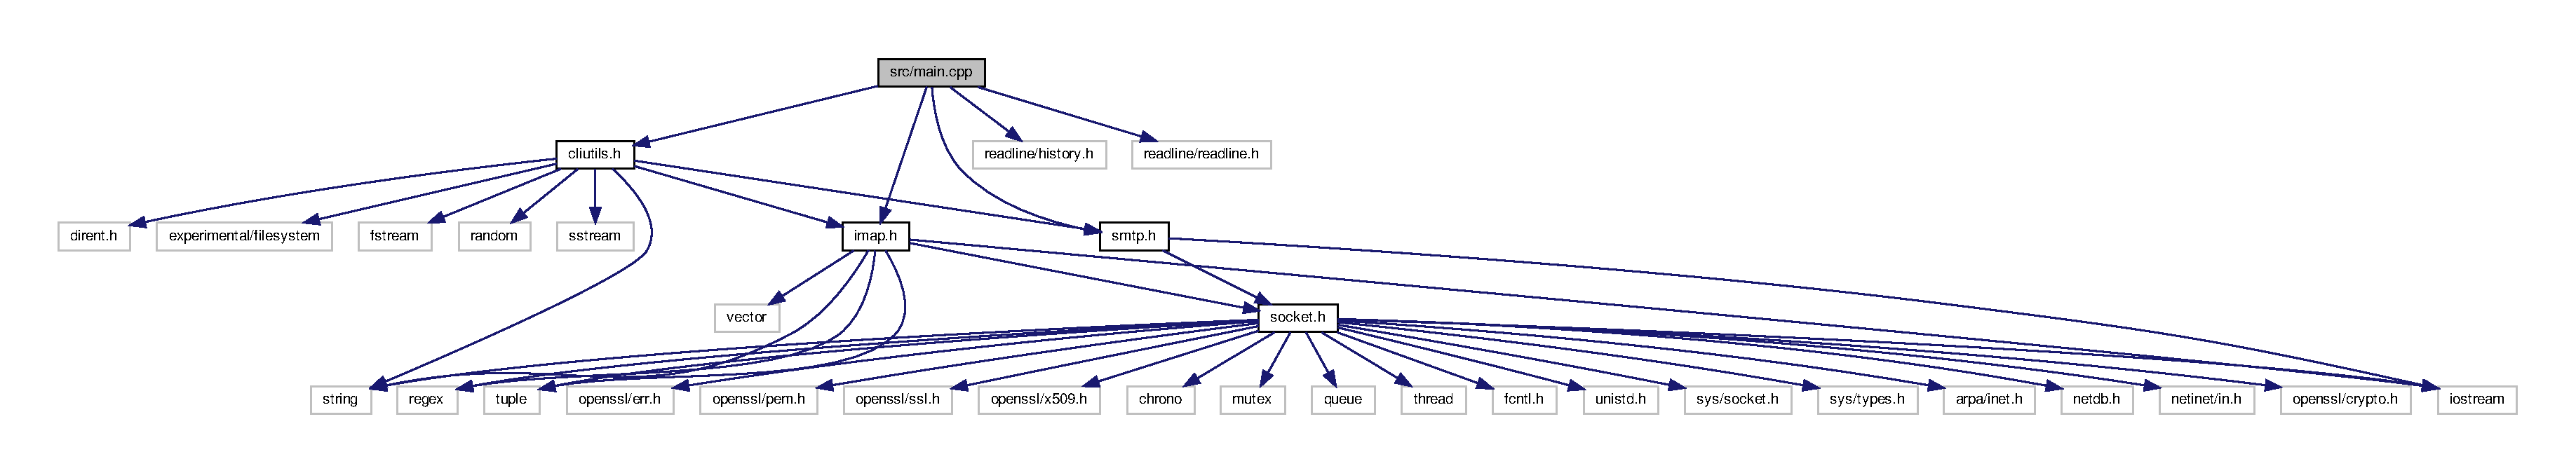
\includegraphics[width=350pt]{main_8cpp__incl}
\end{center}
\end{figure}
\subsection*{Functions}
\begin{DoxyCompactItemize}
\item 
char $\ast$$\ast$ \hyperlink{main_8cpp_a597c9473c751029ee71a0d468862f280}{command\+\_\+completion} (const char $\ast$text, int start, int end)
\begin{DoxyCompactList}\small\item\em Command completion function. \end{DoxyCompactList}\item 
int \hyperlink{main_8cpp_a3c04138a5bfe5d72780bb7e82a18e627}{main} (int argc, char $\ast$$\ast$argv)
\begin{DoxyCompactList}\small\item\em The mail functiom. \end{DoxyCompactList}\item 
char $\ast$ \hyperlink{main_8cpp_a389022a6c7bfb51f750434f0378a0790}{command\+\_\+generator} (const char $\ast$text, int state)
\begin{DoxyCompactList}\small\item\em Generates next possible command. \end{DoxyCompactList}\end{DoxyCompactItemize}
\subsection*{Variables}
\begin{DoxyCompactItemize}
\item 
std\+::vector$<$ std\+::string $>$ \hyperlink{main_8cpp_a31e7caa9c9459b69d95aab5b004c2261}{vocabulory}
\begin{DoxyCompactList}\small\item\em Vocabulory that will be used by readline. \end{DoxyCompactList}\end{DoxyCompactItemize}


\subsection{Function Documentation}
\mbox{\Hypertarget{main_8cpp_a597c9473c751029ee71a0d468862f280}\label{main_8cpp_a597c9473c751029ee71a0d468862f280}} 
\index{main.\+cpp@{main.\+cpp}!command\+\_\+completion@{command\+\_\+completion}}
\index{command\+\_\+completion@{command\+\_\+completion}!main.\+cpp@{main.\+cpp}}
\subsubsection{\texorpdfstring{command\+\_\+completion()}{command\_completion()}}
{\footnotesize\ttfamily char $\ast$$\ast$ command\+\_\+completion (\begin{DoxyParamCaption}\item[{const char $\ast$}]{text,  }\item[{int}]{start,  }\item[{int}]{end }\end{DoxyParamCaption})}



Command completion function. 

This function will be called by readline library


\begin{DoxyParams}{Parameters}
{\em text} & Current text input by user \\
\hline
{\em start} & Start index \\
\hline
{\em end} & End index \\
\hline
\end{DoxyParams}
\begin{DoxyReturn}{Returns}
Array of matching commands 
\end{DoxyReturn}
\mbox{\Hypertarget{main_8cpp_a389022a6c7bfb51f750434f0378a0790}\label{main_8cpp_a389022a6c7bfb51f750434f0378a0790}} 
\index{main.\+cpp@{main.\+cpp}!command\+\_\+generator@{command\+\_\+generator}}
\index{command\+\_\+generator@{command\+\_\+generator}!main.\+cpp@{main.\+cpp}}
\subsubsection{\texorpdfstring{command\+\_\+generator()}{command\_generator()}}
{\footnotesize\ttfamily char$\ast$ command\+\_\+generator (\begin{DoxyParamCaption}\item[{const char $\ast$}]{text,  }\item[{int}]{state }\end{DoxyParamCaption})}



Generates next possible command. 

Generates command that will be used by readline to give suggestion at cli


\begin{DoxyParams}{Parameters}
{\em text} & Text input by user \\
\hline
{\em state} & State of the generator\\
\hline
\end{DoxyParams}
\begin{DoxyReturn}{Returns}
Next possible matching command, null otherwise 
\end{DoxyReturn}
\mbox{\Hypertarget{main_8cpp_a3c04138a5bfe5d72780bb7e82a18e627}\label{main_8cpp_a3c04138a5bfe5d72780bb7e82a18e627}} 
\index{main.\+cpp@{main.\+cpp}!main@{main}}
\index{main@{main}!main.\+cpp@{main.\+cpp}}
\subsubsection{\texorpdfstring{main()}{main()}}
{\footnotesize\ttfamily int main (\begin{DoxyParamCaption}\item[{int}]{argc,  }\item[{char $\ast$$\ast$}]{argv }\end{DoxyParamCaption})}



The mail functiom. 


\begin{DoxyParams}{Parameters}
{\em argc} & Number of cli arguments \\
\hline
{\em argv} & List of cli arguments\\
\hline
\end{DoxyParams}
\begin{DoxyReturn}{Returns}
Returns 0 on exit 
\end{DoxyReturn}


\subsection{Variable Documentation}
\mbox{\Hypertarget{main_8cpp_a31e7caa9c9459b69d95aab5b004c2261}\label{main_8cpp_a31e7caa9c9459b69d95aab5b004c2261}} 
\index{main.\+cpp@{main.\+cpp}!vocabulory@{vocabulory}}
\index{vocabulory@{vocabulory}!main.\+cpp@{main.\+cpp}}
\subsubsection{\texorpdfstring{vocabulory}{vocabulory}}
{\footnotesize\ttfamily std\+::vector$<$std\+::string$>$ vocabulory}

{\bfseries Initial value\+:}
\begin{DoxyCode}
\{\textcolor{stringliteral}{"help"},   \textcolor{stringliteral}{"send"},     \textcolor{stringliteral}{"quit"},   \textcolor{stringliteral}{"read"},
                                    \textcolor{stringliteral}{"search"}, \textcolor{stringliteral}{"delete"},   \textcolor{stringliteral}{"sync"},   \textcolor{stringliteral}{"list"},
                                    \textcolor{stringliteral}{"create"}, \textcolor{stringliteral}{"deletemb"}, \textcolor{stringliteral}{"rename"}, \textcolor{stringliteral}{"move"},
                                    \textcolor{stringliteral}{"noop"}\}
\end{DoxyCode}


Vocabulory that will be used by readline. 


\hypertarget{smtp_8cpp}{}\section{src/smtp.cpp File Reference}
\label{smtp_8cpp}\index{src/smtp.\+cpp@{src/smtp.\+cpp}}
{\ttfamily \#include \char`\"{}smtp.\+h\char`\"{}}\newline
{\ttfamily \#include \char`\"{}utils.\+h\char`\"{}}\newline
Include dependency graph for smtp.\+cpp\+:\nopagebreak
\begin{figure}[H]
\begin{center}
\leavevmode
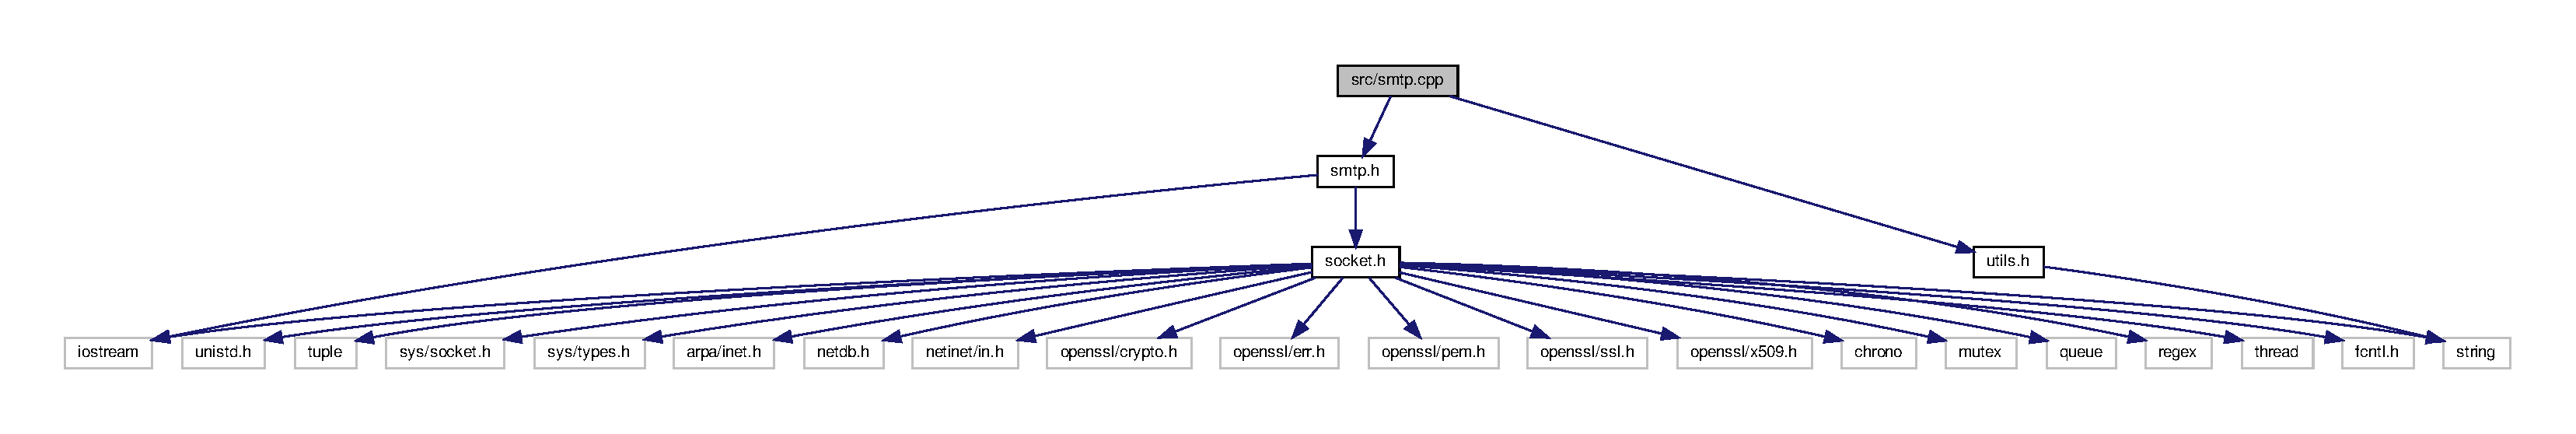
\includegraphics[width=350pt]{smtp_8cpp__incl}
\end{center}
\end{figure}

\hypertarget{socket_8cpp}{}\section{src/socket.cpp File Reference}
\label{socket_8cpp}\index{src/socket.\+cpp@{src/socket.\+cpp}}
{\ttfamily \#include \char`\"{}socket.\+h\char`\"{}}\newline
Include dependency graph for socket.\+cpp\+:
\nopagebreak
\begin{figure}[H]
\begin{center}
\leavevmode
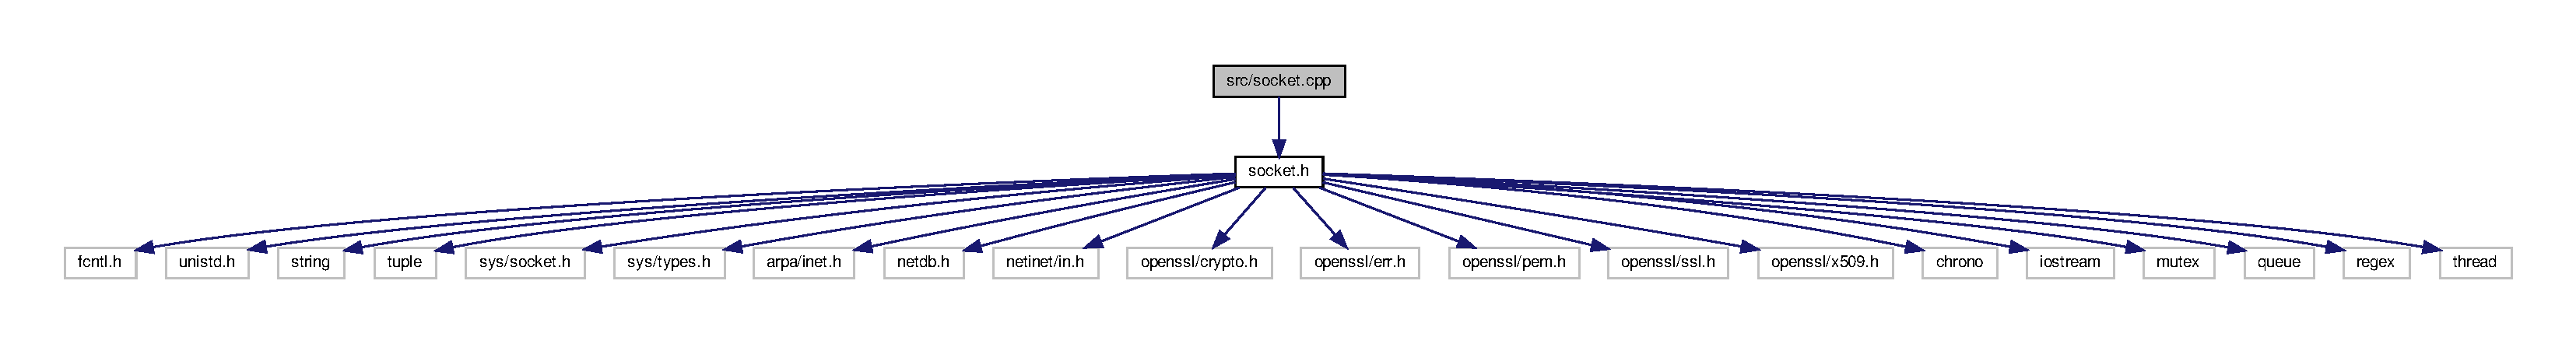
\includegraphics[width=350pt]{socket_8cpp__incl}
\end{center}
\end{figure}

%--- End generated contents ---

% Index
\backmatter
\newpage
\phantomsection
\clearemptydoublepage
\addcontentsline{toc}{chapter}{Index}
\printindex

\end{document}
